\documentclass[11pt]{article}
%\documentclass[ba]{imsart}

\usepackage{fullpage,amsmath}% mathtools}
\usepackage{setspace}
\usepackage{graphicx, psfrag, amsfonts, float}
\usepackage{natbib}
\usepackage{amsthm}
\usepackage{multirow}
\usepackage{hhline}
%\usepackage{color}
\usepackage[position=t,singlelinecheck=off]{subcaption}
\usepackage{caption, setspace}
%\usepackage[position=t,singlelinecheck=off]{subfigure}
 \pdfminorversion=4
\usepackage{rotating}
\def\bgam{\mbox{\boldmath $\gamma$}}
\def\bth{\mbox{\boldmath $\theta$}}
\def\bbeta{\mbox{\boldmath $\beta$}}
\def\blam{\mbox{\boldmath $\lambda$}}
\def\bmu{\mbox{\boldmath $\mu$}}

\newcommand{\bx}{\mbox{\boldmath $x$}}
\newcommand{\bX}{\mbox{\boldmath $X$}}
\newcommand{\bu}{\mbox{\boldmath $u$}}
\newcommand{\bc}{\mbox{\boldmath $c$}}
\newcommand{\bs}{\mbox{\boldmath $s$}}
\newcommand{\by}{\mbox{\boldmath $y$}}
\newcommand{\bz}{\mbox{\boldmath $z$}}
\newcommand{\bv}{\mbox{\boldmath $v$}}
\newcommand{\bb}{\mbox{\boldmath $b$}}
\newcommand{\bzero}{\mbox{\boldmath $0$}}
\newcommand{\thstarj}{\mbox{$\theta^\star_j$}}
\newcommand{\bths}{\mbox{$\btheta^\star$}}
\newcommand{\pkg}[1]{{\fontseries{b}\selectfont #1}} 

\newcommand{\ud}{\mathrm{d}}
\newcommand{\uI}{\mathrm{I}}
\newcommand{\uP}{\mathrm{P}}
\newcommand{\up}{\mathrm{p}}
\newcommand{\mb}{\mathbf}
\newcommand{\mc}{\mathcal}


\newcommand{\Bern}{\mbox{Bern}}
\newcommand{\Nor}{\mbox{N}}
\newcommand{\Ga}{\mbox{Gamma}}
\newcommand{\Dir}{\mbox{Dir}}
\newcommand{\Ber}{\mbox{Ber}}
\newcommand{\Be}{\mbox{Be}}
\newcommand{\Unif}{\mbox{Unif}}
\newcommand{\Binom}{\mbox{Bin}}
\newcommand{\IG}{\mbox{IG}}

\newcommand{\Xs}{X^\star}
\newcommand{\Lc}{{\cal L}}


\usepackage[dvipsnames,usenames]{color}
\newcommand{\yy}{\color{magenta}\it}
\newcommand{\jj}{\color{Black}\rm}
\newcommand{\yjnote}[1]{\footnote{\color{Brown}\rm #1 \color{Black}}}
\newtheorem{theorem}{Theorem}[section]
\newtheorem{definition}[theorem]{\bf Definition}
\newtheorem{lemma}[theorem]{\bf Lemma}
\newtheorem{corollary}[theorem]{\bf Corollary}
\newtheorem{proposition}[theorem]{\bf Proposition}
\newtheorem{assumption}[theorem]{\bf Assumption}
\newtheorem{example}[theorem]{\bf Example}
\newtheorem{remark}[theorem]{\bf Remark}


\newcommand{\iid}{\stackrel{iid}{\sim}}
\newcommand{\indep}{\stackrel{indep}{\sim}}

\doublespacing
\setlength{\textwidth}{6 in}

% commands for for editing
\usepackage{color}
\usepackage{ulem} % \sout
\newcommand{\red}[1]{{\color{red}#1}}
\newcommand{\blue}[1]{{\color{blue}#1}}
\newcommand{\brown}[1]{{\color{brown}#1}}
\newcommand{\green}[1]{{\color{green}#1}}
\newcommand{\magenta}[1]{{\color{magenta}#1}}
\DeclareMathOperator*{\argmin}{\arg\!\min}
\graphicspath{{figures/}}

\makeatletter
\newcommand{\labitem}[2]{%
\def\@itemlabel{\textbf{#1}{.}}
\item
\def\@currentlabel{#1}\label{#2}}
\makeatother

\title{Bayesian Restricted Likelihood Methods: Conditioning on Insufficient Statistics in Bayesian Regression}
\author{John R. Lewis, Steven N. MacEachern and  Yoonkyung Lee \\
{\small \it Department of Statistics, The Ohio State University, Columbus, Ohio 43210}\\
{\small lewis.865@osu.edu, snm@stat.osu.edu and yklee@stat.osu.edu}
\thanks{This research has been supported by Nationwide Insurance Company and by the NSF under grant numbers DMS-1007682 and DMS-1209194.  The views in this paper are not necessarily those of Nationwide Insurance or the NSF.}} 
\begin{document}
\date{}
\maketitle

\begin{abstract}
The \textit{restricted likelihood} is introduced as a method to address concerns about the miss-specification of the likelihood in Bayesian models. To apply, the data is summarized through a set of insufficient statistics,
targeting inferential quantities of interest, and the prior is updated with only the summary statistics. By a careful choice of the summary, we retain the main benefits of Bayesian methods while reducing the
sensitivity of the analysis to features of the data not captured by
the conditioning statistics. Examples specifically address reducing sensitivity to outliers,
where classical robust estimators (e.g., M-estimators) are natural choices
for conditioning statistics. With these choices, the method can be thought of as a blend of classical robust estimation and Bayesian methods. 

A Markov chain Monte Carlo (MCMC) algorithm, applicable for the linear model and a wide range of choices for
summary statistics, is developed to overcome implementation challenges. The method is demonstrated with several examples including simulations and messy insurance agency data with many outliers. Success is manifested in better predictive
performance for data points of interest as compared to competing methods.

\noindent KEYWORDS: Approximate Bayesian computation, Markov chain
Monte Carlo, M-estimation, Robust regression.


\end{abstract}

\section{Introduction}
Bayesian methods are useful to a wide range of scientific problems, with their value
having been demonstrated both empirically and theoretically. However, these methods run into difficulties
for two major and prevalent classes of problems: handling data sets
with outliers and dealing with model misspecification. From Bayesian perspective the model refers to the prior, the likelihood, as well as the loss function when formal inference is required. While optimality of Bayesian methods is unquestioned if one accepts the validity of all three of these elements, healthy skepticism encourages us to question each.  Concern about the prior distribution has
been addressed through objective Bayesian methods \citep{berger2006} prior elicitation methods \citep{garthwaite2005, ohagan2006}. Concern about the loss function is reflected in the extensive literature on Bayesian hypothesis tests \citep{kass1995}.  Despite the common use of flat-tailed distributions \citep{berger1994} or nonparametric techniques \red{References?}, the sampling density has been given less attention from a specifically Bayesian view. The work on predictive diagnostics \citep{box1980} departs from classical
traditions.  

The focus of this work is the development of techniques to handle imperfections in the sampling density.  These imperfections often show
themselves through the presence of outliers--cases not reflecting the phenomenon under
study. There are three main solutions to Bayesian outlier-handling.  The first is to replace the basic sampling
density with a mixture model which includes one component for the ``good'' data and a second 
component for the ``bad'' data.  The second approach replaces the
basic sampling density with a thick-tailed density in an attempt to discount outliers.  The third approach fits a flexible (typically nonparametric) model to the data, producing a Bayesian version of a density estimate for both good and bad data.  In recent 
development, inference is made through the use of robust inference functions \citep[][in press]{lee2013}.  

The traditional strategies for handling outliers all have their drawbacks.  While we view the sampling 
density for the good data as stable, the outlier-generating processes 
may be transitory in nature, constantly shifting as the source of bad data changes.  This prevents
us from appealing to large-sample arguments to claim that, with enough data, we can nail down a
model for both good and bad data combined.  Instead of attempting to model both good and bad
data, we propose a new strategy. In a nutshell, we begin with a complete model   
as if all of the data are good. But rather than driving the move from prior distribution to posterior
distribution by the entire likelihood, we use only the likelihood driven by a
few summary statistics that target inferential quantities
of interest.  We call this the \textit{restricted likelihood}. The update is a formal update from prior distribution to posterior distribution, based on the sampling density of the summary statistics. 

While the focus of this work is handling outliers, model miss-specification is more general. By focusing on robustly estimating quantities of interest and conditioning on these estimates, the restricted likelihood offers promiss in handling more general miss-specification issues in model building. The remainder of the paper.....develops Bayesian restricted likelihood (Section~\ref{restrictedlikelihood}), shows
how it can be applied to a Bayesian linear model (Section~\ref{BayesLinMod}), illustrates its use
on an insurance agencies data set with a novel twist on model evaluation (Section~\ref{Applications}), 
and wraps up with a discussion (Section~\ref{Conclusions}).  
A major contribution of this work is the computational strategy whose legitimacy is established 
in Section~\ref{BayesLinMod}.  The technical proofs are in the appendix.   

\section{The Restricted Likelihood}
\label{restrictedlikelihood}

This sections describes the restricted likelihood using a pair of simple examples and the relates the method to the current literature. For the examples assume $\by=(y_1,\ldots,y_n)$ is a random sample
of size $n$ from a continuous distribution indexed by a parameter
vector $\bth$, with pdf $f(y| \bth)$.  The full-data, likelihood is $L(\bth | \by) = \prod_{i=1}^n f(y_i | \bth)$.  

For the first example, consider that a known subset of the data is not informative about $\bth$.  This case mimics the setting where outlying observations  are identified and discarded before formal analysis. 
Labeling the good cases $1$ through $n-k$ and the bad cases $n-k+1$ through $n$.  
The relevant likelihood to be used to move from prior distribution to posterior distribution is 
$L(\bth | y_1, \ldots, y_{n-k}) = \prod_{i=1}^{n-k} f(y_i | \bth)$.  
Equivalently,  the full 
likelihood is rewritten as 
\begin{eqnarray}
\label{OutlyingCases}
L(\bth | \by)  
= \left( \prod_{i=1}^{n-k} f(y_i | \bth) \right) \left( \prod_{i=n-k+1}^{n} f(y_i | \bth) \right) .  
\end{eqnarray}
The second piece, which is independent of $\theta$,  is dropped to provide better inference on $\bth$.  

A second example involves deliberate censoring of small and large observations.  This is
sometimes done as a precursor to the analysis of reaction time
experiments  \citep[e.g.,][]{ratcliff1993} where very short and long reaction times are usually explained as anticipation and inattention, respectively, and do not reflect the process being studied.
With lower and upper censoring times at $t_1$ and $t_2$, the post-censoring sampling distribution
is of mixed form, with masses $F(t_1|\bth)$ at $t_1$ and $1-F(t_2|\bth)$ at $t_2$,
and density $f(y | \bth)$ for $y \in (t_1, t_2)$.  Adjusting $y_i$,
with $c(y_i)$ where $c(y_i)= t_1$ if $y_i \leq t_1$, $c(y_i)=t_2$ 
if $y_i \geq t_2$, and $c(y_i)=y_i$ otherwise.  
The adjusted update is performed with $L(\bth |c(\by))$.  
With slightly non-standard notation, we let $g(t_1|\bth) = F(t_1|\bth)$,
$g(t_2 | \bth) = 1 - F(t_2|\bth)$, and $g(y|\bth)=f(y|\bth)$ for
$y \in (t_1, t_2)$. The full likelihood as the product of two pieces, 
\begin{eqnarray}
\label{Censoring}
L(\bth | \by) =  \left( \prod_{i=1}^n g(c(y_i)  | \bth) \right) \left( \prod_{i=1}^n f(y_i|\bth,c(y_i) ) \right) ,  
\end{eqnarray}
and only the first for the formal update.  

Further example abound with more given in \cite{lewis2014}. To generalize, we write the full likelihood in two pieces
\begin{eqnarray}
\label{FullLikelihood}
L(\bth | \by)  & = & f(T(\by) | \bth) \,\, f(\by |\bth, T(\by)) .  
\end{eqnarray}
where $T(\by)$ is any statistic. Here,  $f(T(\by) | \bth)$ is the conditional pdf of $T(\by)$ given $\bth$ and $f(\by |\bth, T(\by))$ is the conditional pdf of $\by$ given $\bth$ and $T(\by)$.  In \eqref{OutlyingCases}, the conditioning statistic is $T(\by) = (y_1, \ldots, y_{n-k})$ and in \eqref{Censoring}, the conditioning statistic is $T(\by) = (c(y_1),\ldots,c(y_n))$.  We refer to 
$f(T(\by) | \bth)$ as the restricted likelihood and $L(\bth | \by)=f(\by|\bth)$ as the full likelihood.  

$T(\by)$ is a well-defined random variable with a probability distribution indexed by $\bth$ and the update from prior  to posterior can be made using $f(T(\by)|\bth)$ rather than $f(\by|\bth)$.  This leads to the \textit{restricted likelihood posterior}
\begin{eqnarray}
\label{RestrictedPosterior}
\pi(\bth | T(\by)) & = & \frac{\pi(\bth) f(T(\by) | \bth)}{m(T(\by))} ,
\end{eqnarray}
where $\pi(\bth)$ is the prior distribution and $m(T(\by))$ is the marginal distribution of $T(\by)$ under prior. The associated predictive distribution for a single observation $\tilde y$ is
\begin{eqnarray}
\label{RestrictedpredDist}
f(\tilde y | T(\by)) = \int f(\tilde y | \bth) \pi(\bth | T(\by))\ d\bth .  
\end{eqnarray}

Direct use of restricted likelihood appears in many areas of the literature.  The motivation is often similar to ours:   
concern about outliers or, more generally, model misspecification.  The use of rank likelihoods is discussed by \cite{savage1969}, \cite{pettitt1983, pettitt1982}, and more recently by \cite{hoff2013}.  \cite{lewis2012} make use of robust regression estimators for $T(\by)$.
Asymptotic properties of restricted posteriors are studied by \cite{doksum1990}, \cite{clarke1995}, \cite{yuan2004},  and \cite{hwang2005}. These asymptotic results asserts that under certain assumptions, posterior distribution resembles the asymptotic sampling distribution of the conditioning statistic.  

Restricted likelihoods have been used as practical approximations to a full likelihood. For example, \cite{pratt1965} appeals to heuristic arguments regarding approximate sufficiency to justify the use of the restricted likelihood of the sample mean and standard deviation. Approximate sufficiency is also used in Approximate Bayesian Computation (ABC), which is related to our method.  
ABC has recently experienced success in applications to epidemiology, genetics, and quality control \citep[see, for example,][]{tavare1997, pritchard1999,  marjoram2003, fearnhead2012}. Interest typically lies in the full data posterior and ABC is used for computational convenience.  Consequently, effort is made to choose an approximately sufficient $T(\by)$ and update to the ABC posterior by using the likelihood $L(\bth| \mathcal{B}(\by))$, where $\mathcal{B}(\by)=\{\by^{*}|\rho(T(\by),T(\by^{*}))<\epsilon\}$, $\rho$ is a metric, and $\epsilon$ is a tolerance level. This is the likelihood conditioned on the collection of data sets close to $\by$ as measured by the summary statistic. By choosing an approximately sufficient $T(\cdot)$ and a small enough $\epsilon$ the claim $L(\bth|\mathcal{B}(\by))\approx L(\bth|T(\by))\approx L(\bth|\by)$. Consequently, the ABC posterior approximates the full data posterior. Efforts have been made to formalize what is meant by  approximate sufficiency \citep[e.g.,][]{joyce2008}.

ABC is related to our method in that conditioning is on something other than the full data. For technical reasons, the calculation proceeding from $\pi(\bth)$ to $\pi(\bth | \mathcal{B}(\by))$ is not a formal conditional update.  Simply put, if an external observer told $\mathcal{B}(\by)$ can supply $T(\by)$ and vice-versa, the information contained in $\mathcal{B}(\by)$ is exactly that contained in $T(\by)$ and proper conditioning will lead to identical posterior distributions.  This is not the case with a typical implementation of ABC.  

% In a related, but distinctly different, approach which also takes advantage of summary statistics, the full data log likelihood is replaced by a loss function \citep[e.g.][]{bissiri2013} in an effort to concentrate inference only on parameters of interest. In contrast, the incomplete likelihood is formulated using a full probability model, allowing for a formal Bayesian update, while remaining robust to misspecification.

This work extends the development of Bayesian restricted likelihood by arguing that deliberate choice of $T(\by)$ is sound practice and also by expanding the class of conditioning statistics in which exact conditioning can be achieved. Our methods do not rely on asymptotic properties, approximate conditioning, nor do they need to correspond to artificial censoring to create incomplete or missing data \citep[e.g.,][]{albert1988, hoffwakefield2013}.  \green{Note - fix references here hoffwakefield for asymptotic; albert for ? .}  

\red{ MOVE THIS PIECE OR REMOVE ---
The key to productive use of the restricted likelihood is the choice of $T(\by)$ and the development
of computational strategies that allow us to truly condition on the observed $T(\by)$ and 
fit the model in formal Bayesian fashion.  In this work, we focus
on robustness, and natural choices of $T(\by)$ for the one-sample problem include a set of middling order statistics, a trimmed
mean, or a classical robust estimator of location and/or scale.  
We have previously implemented several of these methods and have found them to perform well \citep[][]{lewis2012}. Versions most extensible to the linear model include the M-estimators in the tradition of \cite{huber1964}, least median squares (LMS), and least trimmed squares (LTS). For these choices the restricted likelihood is not available in closed form, making computation of the restricted posterior a challenge. For low-dimensional statistics $T(\by)$ and parameters $\bth$, the direct computational strategies described in \cite{lewis2014} can be used to estimate the incomplete posterior conditioned on essentially any statistic.  These strategies rely on generation of complete data sets from different values of $\bth$.  
Each complete data set leads to a statistic $T(\by)$ under $\bth$, and these generated statistics are used to estimate the density at $T(\by_{obs})$, where $\by_{obs}$ is the observed complete data. This estimate is fed into Bayes' theorem for the update from prior distribution to posterior distribution.  %For the example in the previous section, these strategies work well.
%\textcolor{blue}{Comment out `A variety of  variance reduction techniques which exploit\dots' because it seemed too vague and a bit off topic}
%In low dimensional settings (in $T(\by)$ and $\bth$) the incomplete posterior under each of these versions (and others) can be estimated by approximating the incomplete likelihood using kernel density estimation techniques \citep[for details see][]{lewis2014}. 

These direct sampling techniques rely on density estimation and numerical integration. Density estimation becomes difficult for high dimensional $T(\by)$ and numerical integration breaks down for high dimensional $\bth$. For these settings, an MCMC algorithm is developed in Section \ref{highDim}. Software is available from the authors for use with simultaneous M-estimators of location and scale. At the present time, further software development is required to extend beyond simultaneous M-estimators.  

%\textcolor{blue}{Added a bit about this to the discussion: Though we concentrate in this paper on applying incomplete likelihood inference for the mean of linear regression models, the computational strategies we devise in subsequent sections also allow us to apply the method to inference beyond the mean.  In particular, quantile regression falls within the framework we develop. }
%The next section develops the necessary computational strategies.  
}

\section{Examples}
\label{examples}
Before discussing computational details, the method is applied to two simple examples on well known datasets to demonstrate its effectiveness in situations where outliers are a major concern. The full model in each case fits into the Bayesian linear regression framework discussed in \ref{}. Specific details are left to the Appendix. 

The first example is an analysis of Simon Necomb's 66 measurements of the speed of light; two of which are significant outliers in the lower tail. The full model is a standard location-scale Bayesian model assuming normally distributed errors. Four versions of the restricted likelihood are fit with conditioning statistics: 1) Huber's M-estimator for location with Huber's `proposal 2'  for scale 2)   Tukey's M-estimator for location with Huber's `proposal 2'  for scale 3) LMS (least median squares) for location with associated estimator of scale and 4) LTS (least trimmed squares)  for location with associated estimator of scale. Additionally, the common approach of assuming a t-distribution for the errors is also fit. The posteriors of $\beta$ under each model appear in Figure \ref{fig:newcomb_beta}. As expected, the posterior under the normal model is pulled downward by the two outliers while the heavy tailed model provides robustness against them. The restricted likelihood methods using the M-estimators and LTS statistics also achieve robustness against the outliers. Conditioning on LMS however, results in a posterior similar to the one under the normal model. The M-estimators provide the tightest posteriors in this case. They also provide more precise predictions than the heavy-tailed model as illustrated by the predictive distributions displayed in \ref{fig:newcomb_predictive} which are also dependent on the posterior for the scale parameter.


\begin{figure}
\centering
\begin{subfigure}{.45\textwidth}
{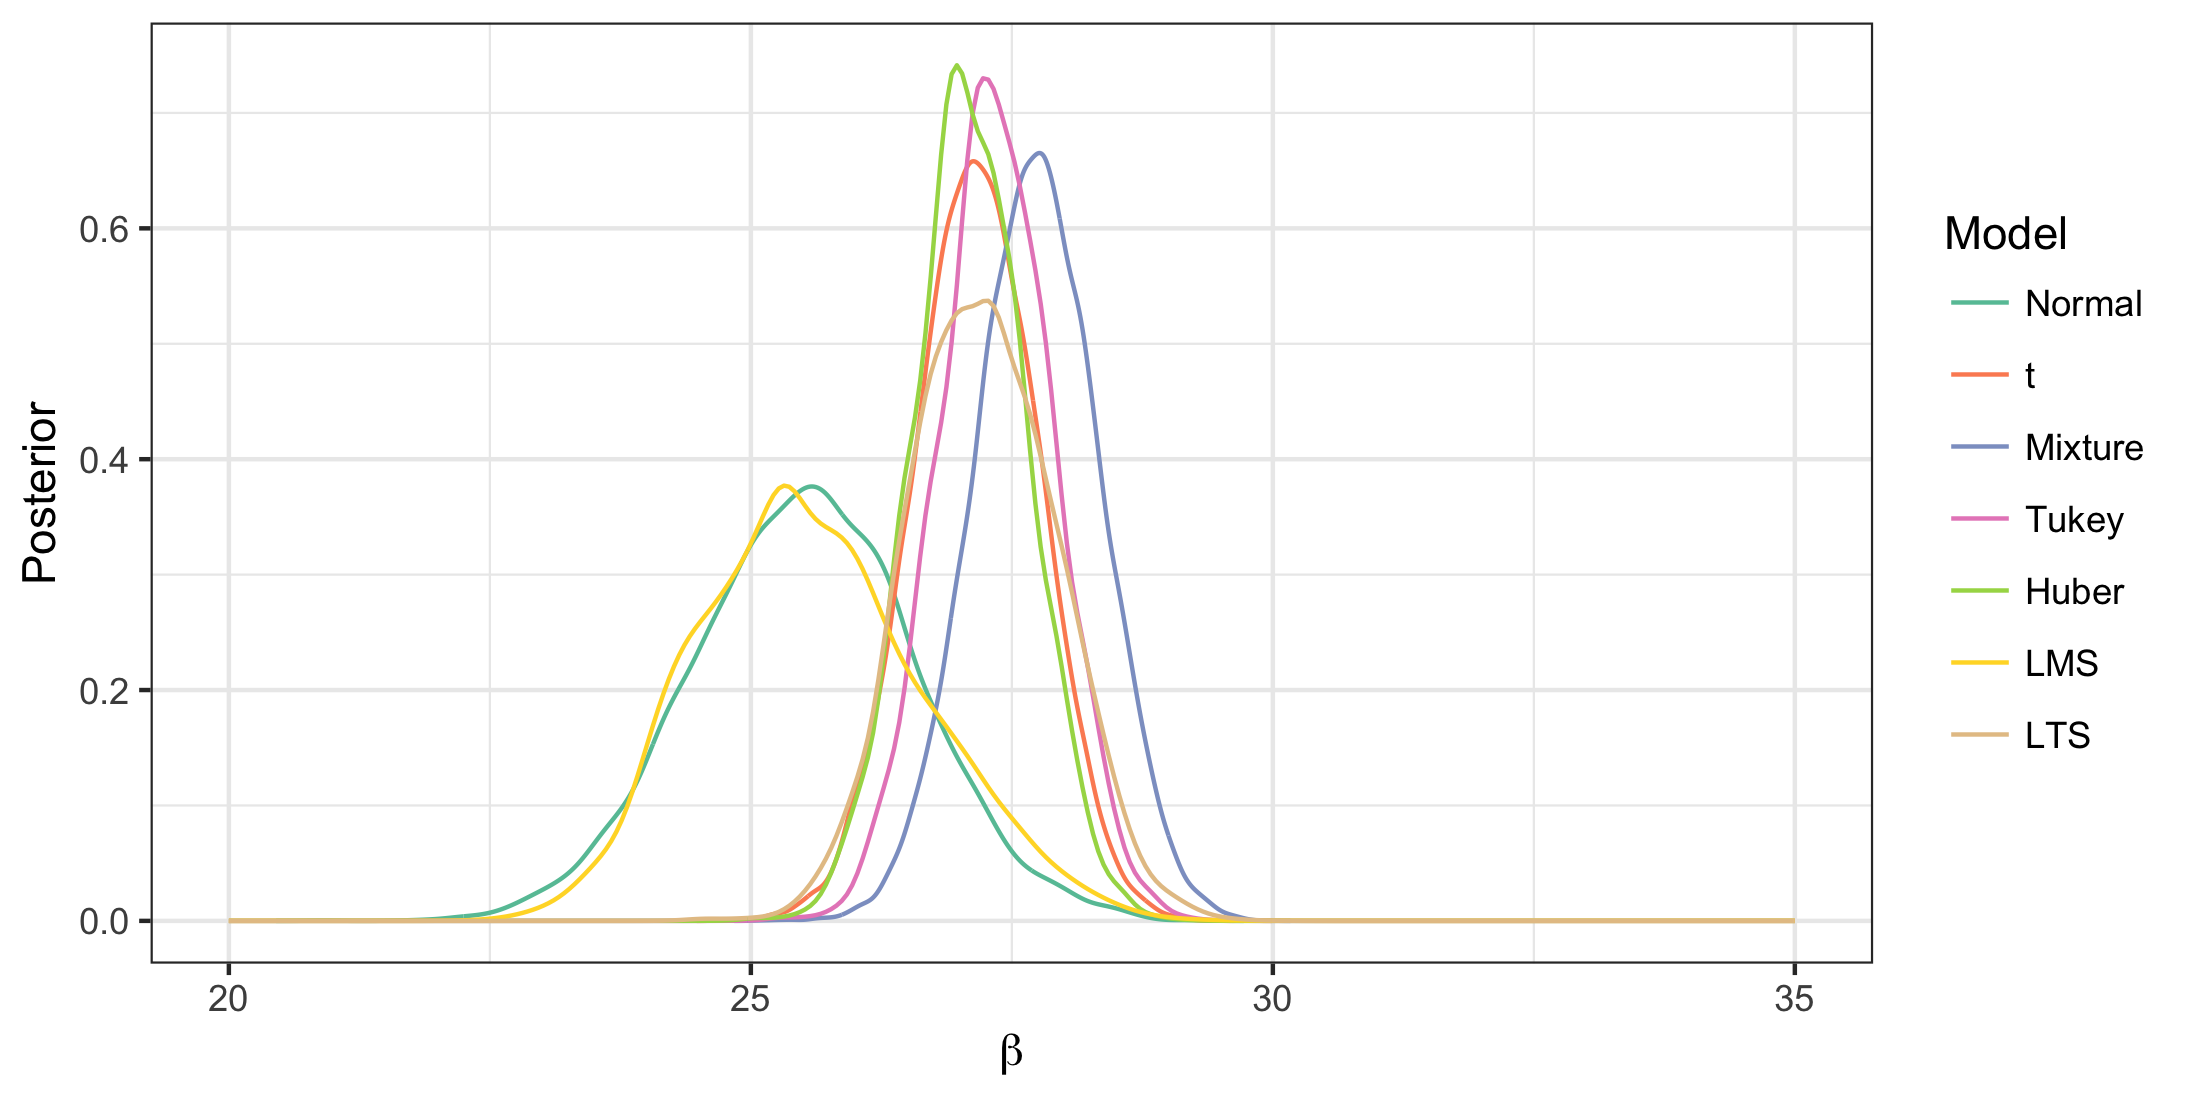
\includegraphics[width = 3.1in]{figs/speed_of_light_beta.png}}
\caption{Posteriors of the location parameter $\beta$ under the normal theory model, the t-model, and four restricted likelihood models for Newcomb's speed of light measurements.}
\label{fig:newcomb_beta}
\end{subfigure}
\begin{subfigure}{.45\textwidth}
\centering
{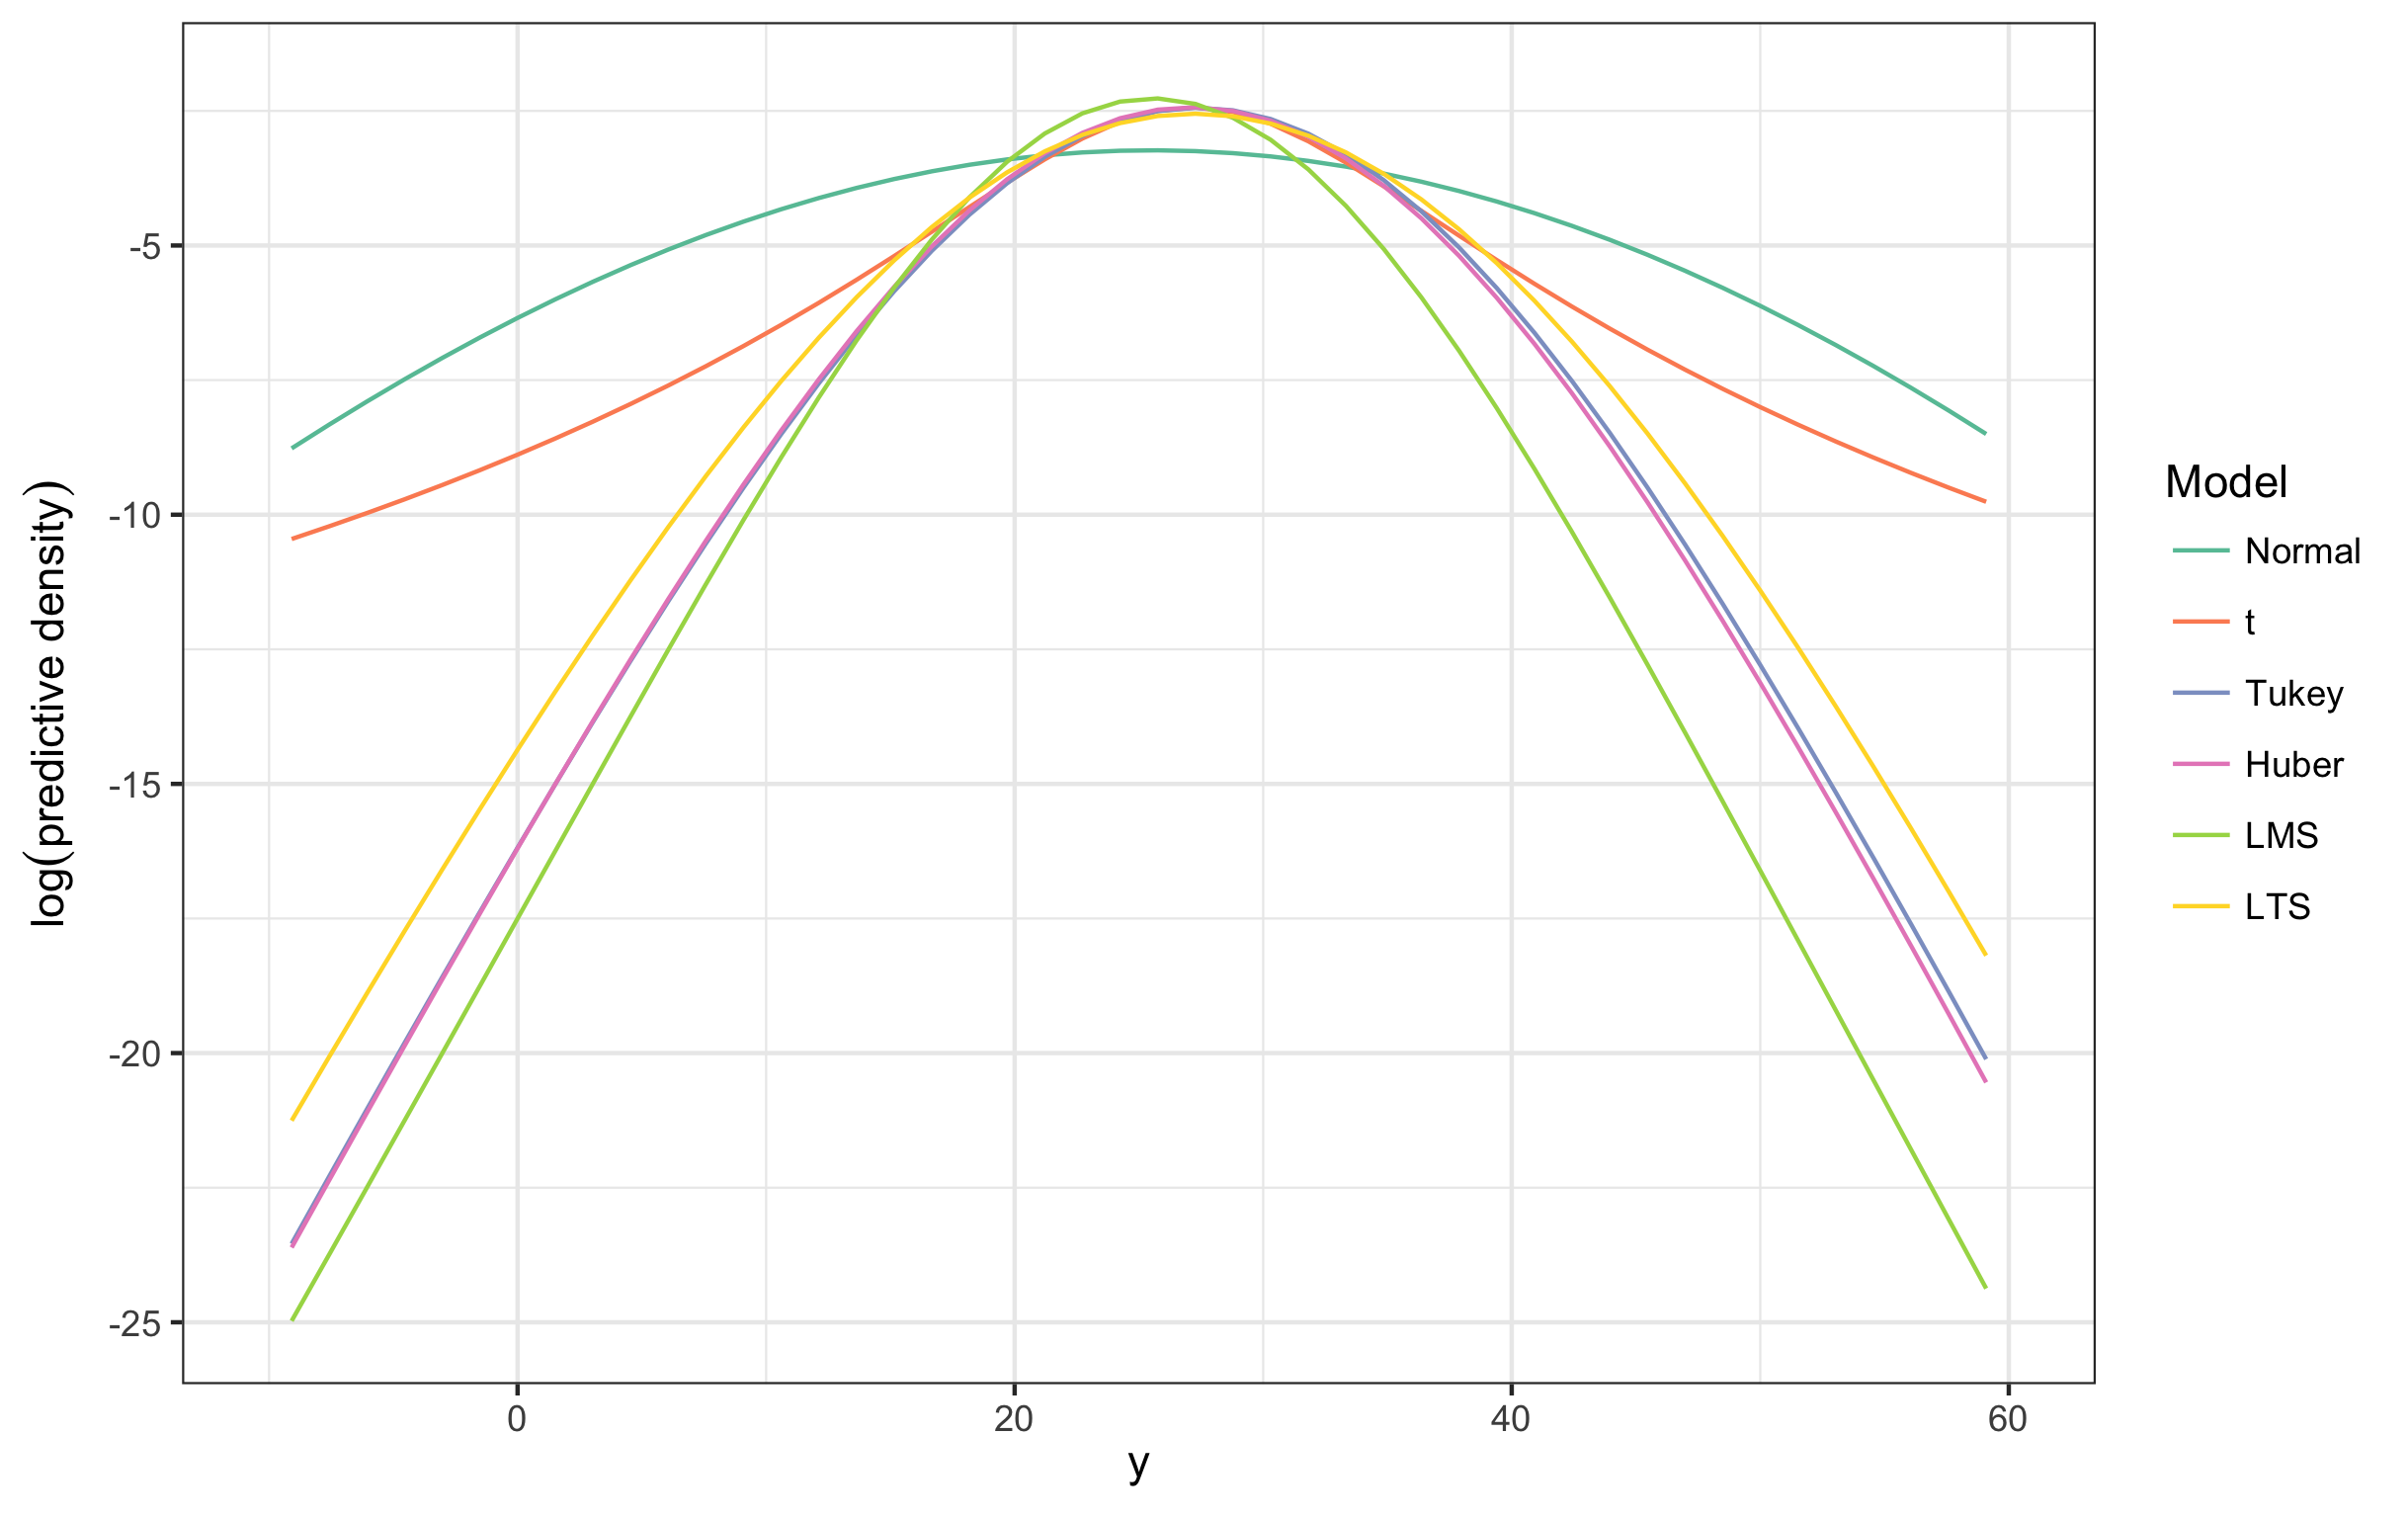
\includegraphics[width = 3.1in]{figs/speed_of_light_predictive.png}}
\caption{Posterior predictive distribution of the speed of light under the normal theory model, the t-model, and four restricted likelihood models.}
\label{fig:newcomb_predictive}
\end{subfigure}
\caption{}
\end{figure}



As a second example, the phones dataset measuring the number of telephone calls in Belgium from 1950-1973 is analyzed. The outliers in this case were due simply to a change in units on which calls were recorded for part of the dataset. The full model is a standard normal Bayesian linear regression with year as the only covariate and response the logarithm of the number of calls. The restricted likelihood method uses Tukey's M-estimator for the slope and intercept with Huber's `proposal 2'  for scale. Likewise, the heavy-tailed t-distribution model is fit. The data along with  $95\%$ credible bands of the posterior predictive distribution under each model are displayed in Figure \ref{}. The normal theory model is only fit to the obvious non-outlying points. Since the t-model assumes the data are heavy-tailed, the posterior predictive distribution is much wider. Further, the outliers are not symmetric as assumed by this model, resulting in the posterior being pulled toward the outliers. On the other hand, the predictive distribution under the restricted likelihood approach is much more precise and is close to that of the normal theory fit that discards the outliers. Alternatively, a two component mixture distribution could also be used with one component for the `good' data and another for the outliers. The predictive distribution would then just use the component for the good data. This would work in this case, but involves explicitly modeling the outlier generating mechanism. In more more complex situations where the outlier generating mechanism is transient (i.e. ever changing and more complex than just a unit error in the recording), modeling the outliers becomes more difficult. Like classical robust estimation, the restricted likelihood approach avoids explicitly modeling the outliers. 

\begin{figure}
\centering
{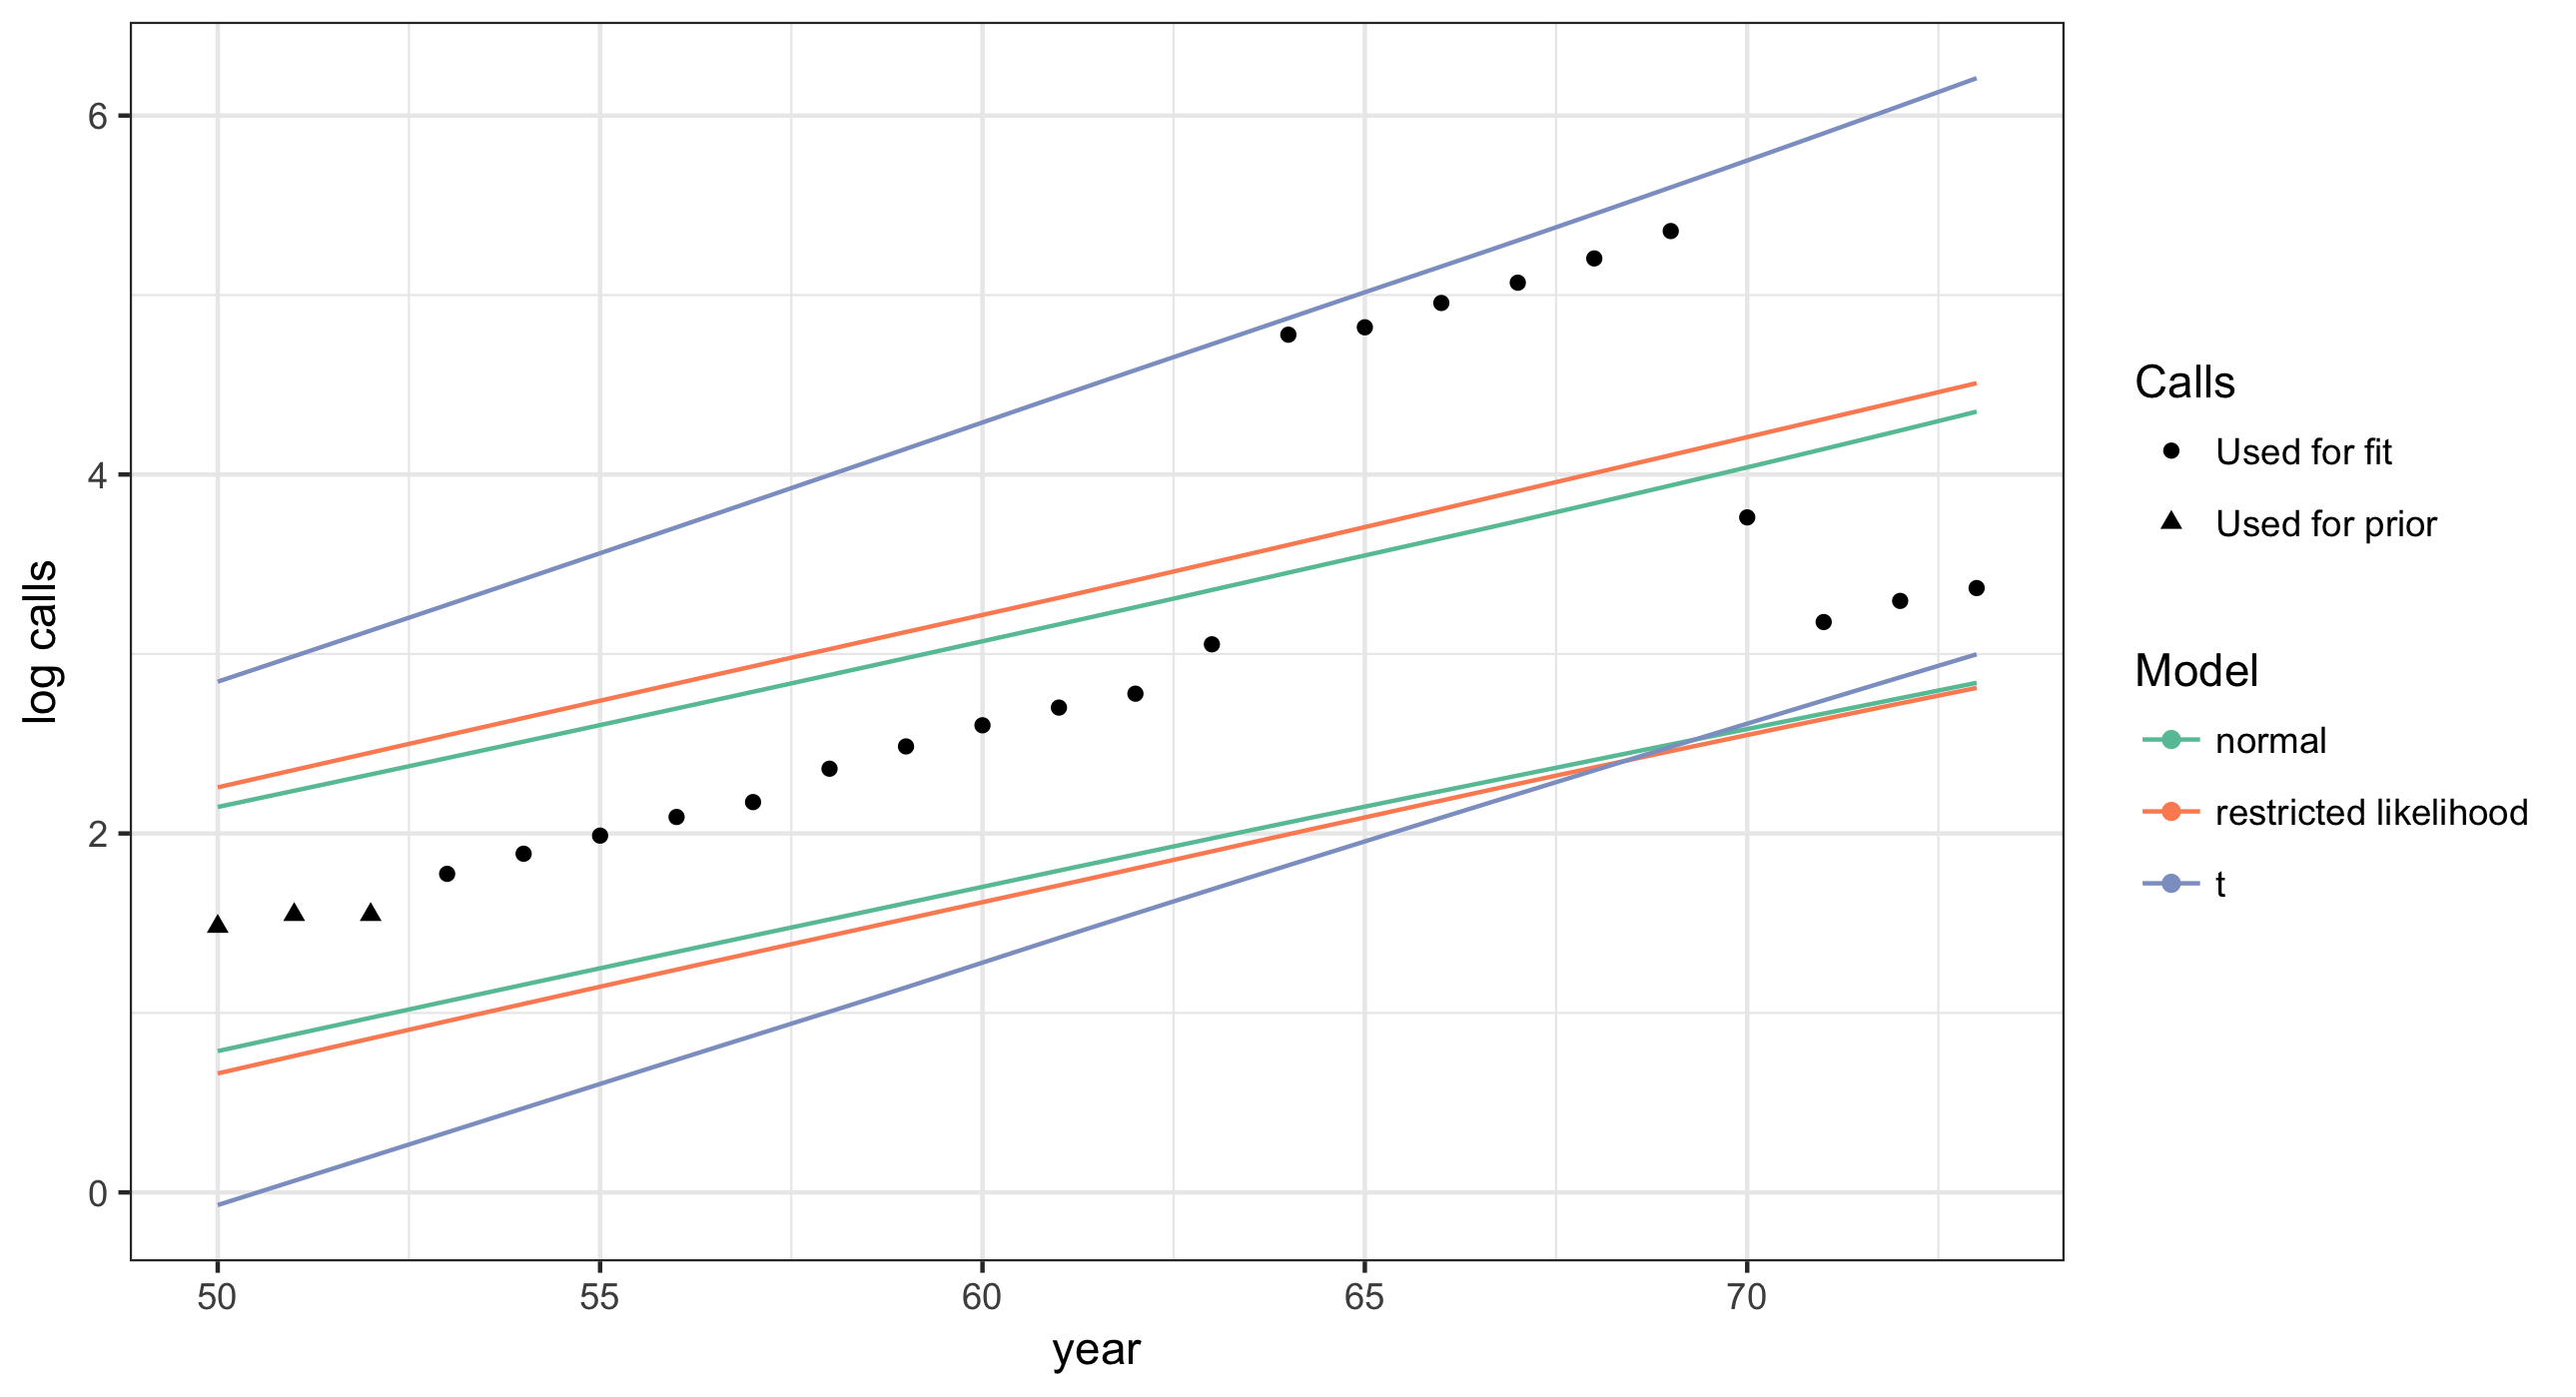
\includegraphics[width = 4in]{figs/calls_predictive.png}}
\label{fig:calls_predictive}
\caption{Predictive distribution of log(calls) under the Normal theory model fit to the non-outliers, the restricted likelihood model with  Tukey's M-estimator for the slope and intercept with Huber's `proposal 2'  for scale, and a heavy-tailed t-distribution model. The first three data points were used to specify the prior with the remaining points used in the posterior fits. See details in the Appendix. }
\end{figure}



\section{Restricted Likelihood for the Linear Model}
\label{BayesLinMod}

\subsection{The Bayesian linear model}
We focus on the use of restricted likelihood for the Bayesian linear
model: 
\begin{eqnarray}
\label{LinearModel}
\bth&=&(\bbeta,\sigma^2) \sim  \pi(\bth) 
\nonumber\\
y_i  & =  & x_i^\top \bbeta + \epsilon_i , \mbox{ for } i = 1, \ldots, n 
\end{eqnarray}
where $x_i$ and $\bbeta \in \mathbb{R}^p$, $\sigma^2 \in \mathbb{R}^+$, 
and the $\epsilon_i$ are independent 
draws from a distribution with center $0$ and scale $\sigma$.
Two conditions are imposed on the model:
\begin{itemize}
\labitem{C1}{fullRank} The $n \times p$ design matrix, $X$, whose $i^{th}$ row is $x_i^\top$, 
is of full column rank.  
\labitem{C2}{supReal} The $\epsilon_i$ are a random sample from some distribution which has a density with 
respect to Lebesgue measure on the real line and for which the support is the real line.  
\end{itemize}

%\textcolor{blue}{commented out `Both conditions can be relaxed, although this would necessitate restating several later results.' and the paragraph here starting with `in the sequel'}
%In the sequel, we specifically consider both normal and $t$ distributions with
%mean $0$ and variance $\sigma^2$ for the $\epsilon_i$ 
%but note that our methods apply much more widely.  The prior distributions $\pi_1$ and $\pi_2$ can take
%many forms and may be joined to form a joint distribution for non-independent $\bbeta$
%and $\sigma^2$.  The conditionally conjugate normal/inverse gamma pair is a common 
%choice.  
%The methods we develop apply to the linear model in \eqref{LinearModel} and to many variations
%on it. For example, the prior distributions $\pi_1$ and $\pi_2$ can be joined to form a joint distribution for non-independent $\bbeta$
%and $\sigma^2$. 
As summary statistics for the data, we concentrate on robust estimators for the 
regression coefficients in the linear model and an associated 
estimator of the scale. In particular, we demonstrate the method using simultaneous M-estimators \cite{} or add equations. The estimator of the regression coefficients is denoted by $\bb(X, \by)\in \mathbb R^{p}$ and that of the scale by $s(X, \by)\in \{0\} \cup {\mathbb R}^+$ . Thus, $T(\by)=(\bb(X, \by), s(X, \by))$. The observed complete data is denoted by $\by_{obs}$ with observed statistic  denoted by $T(\by_{obs})=(\bb(X, \by_{obs}), s(X, \by_{obs}))$. %Assumption \ref{supReal} is important as it translates into a continuous distribution for $\bb(X, \by)$ and $s(X, \by)$ (with respect to $\by$), which is presumed for our computational strategy described below. The full column rank assumption \ref{fullRank} is made apparent by an examination of the proofs in the the appendix. 

%These estimates convey information about $\bth=(\bbeta,\sigma)$
%while downweighting outliers.  The M-estimator of $\bbeta$ is determined by a $\rho$ function through the minimization
%\begin{eqnarray}
%\label{Mest}
%\bb(X,\by) & = & \argmin_{\bbeta} \sum_{i=1}^n \rho\left(\frac{y_i - x_i^\top \bbeta}{\sigma}\right) .  
%\end{eqnarray} 
%The scale estimator $s(X,\by)$ is determined simultaneously as another M-estimator or is determined through
%a separate calculation, for example the mean-absolute-deviation from an $\ell_1$ regression fit. Other estimators for the coefficients considered are least median squares (LMS) and least trimmed squares (LTS). LMS minimizes the median squared residual and LTS minimizes the sum of the $k$ smallest squared residuals where $k$ is chosen by the user. These estimators are also coupled with a scale estimator.% that is determined by the objective function evaluated at the minimum, appropriately scaled by a correction factor for consistency. 

%which is presumed for our computational strategy. %Before deriving this strategy in section \ref{highDim}, we demonstrate the utility of the incomplete likelihood with a simple location and scale example. %The results we derive also apply to other estimators satisfying conditions \ref{asb}-\ref{scaleEq2Reg} below, not just M-estimators.   



\subsection{Computational strategy}
\label{highDim}
%For low-dimensional statistics $T(\by)$ and $\bth$, the direct computational strategies described in \cite{lewis2014} can be used to evaluate the incomplete likelihood posterior.  
%These strategies rely on generation of complete data sets from different values of $\bth$.  
%Each complete data set leads to a statistic $T(\by)$ under $\bth$, and these generated statistics are used to estimate the density at $T(\by_{obs})$, where $\by_{obs}$ is the observed complete data. This estimate is fed into Bayes' theorem for the update from prior distribution to posterior distribution.  For the example in the previous section, these strategies work well.
%\textcolor{blue}{Comment out `A variety of  variance reduction techniques which exploit\dots' because it seemed too vague and a bit off topic}
%A variety of  variance reduction techniques which exploit 
%properties of the distribution of $\by$ 
%improve the performance of these strategies.  

Computational strategies to approximate the restricted posterior involving kernel density estimation and numerical integration are discussed in \cite{}. Such methods break down for high-dimensional statistics $T(\by)$ or high-dimensional parameters $\bth$. This section describes a Markov chain Monte Carlo (MCMC) algorithm which overcomes these limitations for a wide class of conditioning statistics  $T(\by)$. 

The general approach is a data augmented
MCMC algorithm targeting $f(\bth, \by |
T(\by)=T(\by_{obs}))$, the joint distribution of $\bth$ and the full
data given the summary statistic $T(\by_{obs})$. 
The Gibbs sampler \citep{gelfand1990} iteratively samples from the full conditionals $\pi(\bth|\by, T(\by)=T(\by_{obs}))$ and $f(\by|\bth, T(\by)=T(\by_{obs}))$.  Alternative algorithms substitute other generations for the full conditionals, such as the Metropolis-Hastings propose and accept/reject framework.  Our algorithms are based on the decomposition of the MCMC algorithm into conventional full data sampling steps where $\bth$ is generated given $\by$, and steps that allow us to complete the data set where $\by$ is generated given $\bth$ and $T(\by)$.  The latter generation relies on the conditioning set $\mathcal{A}=\{\by\in \mathbb{R}^n|T(\by)=T(\by_{obs})\}$.  The set $\mathcal{A}$ may contain more than one element (i.e., it is not degenerate) when $T(\by) : \by \rightarrow T(\by)$ is not a $1-1$ function.
 
When $\by$ has the summary statistic matching $T(\by_{obs})$, $T(\by) = T(\by_{obs})$,
the first full conditional, $\pi(\bth|\by, T(\by)=T(\by_{obs}))$, is
the same as the full data posterior
$\pi(\bth|\by)$. In this case, the condition $T(\by) = T(\by_{obs})$ is redundant.  This allows us to make use of conventional MCMC steps for this generation.  For typical regression models, algorithms for this step are readily available.  %Recommended algorithms depend on details of the prior distribution and sampling density.  As examples, a normal prior distribution and normal likelihood in the regression setting allow one to alternate conditional generations of $\sigma^2$ and $\bbeta$, and blocking the generation of $\bbeta$ generally leads to quicker convergence and mixing \citep{liu1994}; a thick-tailed scale mixture of normal distributions in the style of the hyper-$g/n$ prior \citep{liang2008} necessitates an additional stage for the sampler where the scale  $g/n$ is generated; a thick-tailed sampling density such as a $t$ distribution can be handled with the addition of a scale parameter for each case and an extra stage where these scale parameters are generated.  

For a typical model and conditioning statistic, the second full conditional $f(\by|\bth, T(\by)=T(\by_{obs})) =f(\by|\bth, \by\in\mc A)$ is not available in closed form.  As a consequence, we turn to Metropolis-Hastings \citep{hastings1970},
using the strategy of proposing full data $\by$ such that $T(\by) = T(\by_{obs})$ and either accepting or rejecting the
proposal. Let $\by_p$ and  $\by_c$ represent the proposed and current
full data, respectively, both belonging to the set $\mathcal{A}$. Denote the proposal distribution for $\by_{p}$ by $p(\by_p|\bth,T(\by_p) = T(\by_{obs}))  = p(\by_p|\bth,\by_p \in \mathcal{A}) = p(\by_p | \bth)$.  The last equality follows from the fact that our $p(\cdot | \bth)$ assigns probability one to the event $\{ \by_p \in \mathcal{A} \}$.  These equalities still hold if the dummy argument $\by_p$ is replaced with $\by_c$.  The conditional density is
\begin{eqnarray*}
f(\by | \bth, \by \in \mathcal{A}) & = & \frac{f(\by | \bth) I(\by \in \mathcal{A} | \by, \bth)}{\int_\mathcal{A} f(\by | \bth) d\by} \\
     & = & \frac{f(\by | \bth)}{\int_\mathcal{A} f(\by | \bth) d\by} 
\end{eqnarray*}
for $\by \in \mathcal{A}$.   


The Metropolis-Hastings acceptance probability  is the minimum of 1 and $R$ where,
\begin{eqnarray}
\label{MHRatio}
R & = & \frac{f(\by_p|\bth,\by_p \in \mathcal{A})}{f(\by_c|\bth,\by_c \in \mathcal{A})}  
                \green{\frac{p(\by_c|\bth, \by_c \in \mathcal{A})}{p(\by_p|\bth,\by_p \in \mathcal{A})}} \\
  & = & \frac{f(\by_p | \bth)}{\int_\mathcal{A} f(\by | \bth) d\by} \frac{\int_\mathcal{A} f(\by | \bth) d\by}{f(\by_c | \bth)} \frac{p(\by_c | \bth)}{p(\by_p | \bth)} \\
 & = & \frac{f(\by_p|\bth)}{f(\by_c|\bth)} \frac{p(\by_c|\bth)}{p(\by_p|\bth)} .  
\end{eqnarray}
\green{Note:  Above expression changed.  Check argument again.}
%In the above expression, the second line follows from the first for
%the following reason. The proposed \green{vector $\by$} is sampled from
%  $\mathcal{A}$ so that
%$T(\by_{p})=T(\by_{c})=T(\by_{obs})$. This implies 
%\green{\sout{$f(\by |\bth,
%T(\by)=T(\by_{obs}))=f(\by |\bth)\pi(\bth)/\red{f[?]}\pi(\bth, T(\by)=T(\by_{obs}))$}
%\begin{eqnarray}
%f(\by |\bth,\by \in \mathcal{A})) & = & \frac{f(\by | \bth) \pi(\bth) I(\by \in \mathcal{A})}{\int f(\by | \bth) \pi(\bth) I(\by \in \mathcal{A}) d\bth}
%\end{eqnarray}}
%where $\by$ represents either $\by_{p}$ or $\by_{c}$. %Further, the expressions $\pi(\bth)$ and $\red{f[?]}\pi(\bth, T(\by)=T(\by_{obs}))$ 
%\green{The expressions $\pi(\bth)$ and $\int f(\by | \bth) \pi(\bth) I(\by \in \mathcal{A})  d\bth$} are the same for $\by_{p}$ and $\by_{c}$ and cancel in the ratio. %Similar expansions can be made for the proposal distribution. 
%\green{Further, the indicator functions can be dropped since $\by_p$ and $\by_c$ will both fall in $\mathcal{A}$.}  
%\green{Note:  Check this argument carefully}

For the models we consider, evaluation of $f(\by | \bth)$ is straightforward.  Therefore, the difficulty in implementing this Metropolis-Hastings step manifests  itself in the ability to simulate proposals that guarantee $T(\by) = T(\by_{obs})$ and on the evaluation of the proposal density derived from the method used to simulate $\by$. We now discuss such an implementation method for the linear model in \eqref{LinearModel}.

\subsubsection{Construction of the proposal}
%\textcolor{blue}{some major revisions as indicated in the responseToReferees}
Our computational strategy is easiest to envision in a location-scale setting where 
the design matrix in model (\ref{LinearModel}) consists of a single column of ones.  Robust estimation techniques along
with model (\ref{LinearModel}) suggest a conditioning statistic $T(\by)$ which consists of
estimates of the scalars $\beta$ and $\sigma$, say $T(\by)=(b(X,\by),
s(X,\by))$.  It is not a simple matter to directly sample the required
proposal $\by$ satisfying $T(\by)=T(\by_{obs})$. However, 
  with equivariance/invariance properties of $T(\by)$, we will see in Theorem \ref{Transformation} below
    that it is possible to scale and shift any \sout{$\bz^{*}\in \mathbb R^{n}$} \green{$\bz^{*}$ which generates 
a positive scale estimate} to such a
    $\by$. Hence, to obtain $\by$ from $\mathcal A$, we proceed
  in two steps. First, a vector $\bz^*$ is sampled from a known
  distribution (examples of which are described later). This vector has summary statistic   
$T(\bz^*) = (b(X,\bz^*), s(X,\bz^*))$.  Second, $\bz^*$ is mapped into $\by =h(\bz^*)$
using Theorem \ref{Transformation} so that $T(\by)=T(\by_{obs})$. To
evaluate the proposal density $p(\by|\bth)$, we need to adjust
the known density of $\bz^*$, $p(\bz^*)$, with the Jacobian of
the transformation $h(\cdot)$ to $\by$. We choose the
distribution of the \green{\sout{intermediate}} data vector $\bz^*$ to have support
\green{on a subset of $\mathbb R^n$ so that}
the transformation to $\by$ is one-to-one and the Jacobian,
$\displaystyle \left|\frac{\partial h^{-1}(\by)}{\partial \by}\right|$, can be computed from first principles. It is the calculation of this Jacobian which is described in the section. We will repeatedly return to an artificial low-dimensional example in the location-scale setting to help visualize this calculation.  

% To 
%obtain data $\by$ for which $T(\by) = T(\by_{obs})$, we proceed in two
%steps.  
%First, a vector $\bz^*$ is generated from a simple manifold with known
%density, for example, a uniform distribution
%on the surface of the unit sphere in ${\mathbb R}^{n-1}$ (alternatively from
%the model with current values of $\beta$ and $\sigma$).  This leads to 
%$T(\bz^*) = (b(X,\bz^*), s(X,\bz^*))$.  The vector $\bz^*$ is mapped into a vector
%$\by$ by rescaling and shifting appropriately to match the observed conditioning statistic.  For typical estimators, the appropriate scaling is 
%$s(X,\by_{obs}) / s(X,\bz^*)$ with the shift trailing along as needed to match $b(X,\by_{obs})$.  
%To evaluate the proposal density of $\by$,
%we need to adjust the density of $\bz^*$ with a Jacobian.  In the sequel, we use this artificially low-dimensional
%example to illustrate the method.  

The strategy described in the previous paragraph extends to full-blown regression models.  Robust regression methods lead naturally to a conditioning statistic in the form of a classical M-estimator for $\bbeta$
and a companion estimator for $\sigma$.  We denote the resulting estimator which involves the covariates through
the design matrix and the response 
as $T(\by) = (\bb(X,\by), s(X,\by))$, with $\bb(X,\by) = (b_1(X,\by), \cdots,
b_p(X,\by))^\top$.  Simultaneous M-estimators have a number of standard properties \ref{asb}-\ref{scaleEq2Reg} which
prove useful in the sequel \citep{huber2009, maronna2006}.  
\begin{itemize}
\labitem{C3}{asb}$\bb(X,\by)$ is almost surely continuous and differentiable with respect to $\by$.  
\labitem{C4}{as} $s(X,\by)$ is almost surely positive, continuous, and differentiable with respect to $\by$.  
\labitem{C5}{regEq} $\bb(X,\by+X\bv)=\bb(X,\by)+\bv \ \ \text{for  all}\ \bv\in\mathbb{R}^p$. 
\labitem{C6}{scaleEqReg} $\bb(X,a\by)=a\bb(X,\by)\ \ \ \text{for all constants } a$.  
\labitem{C7}{regIn} $s(X,\by+X\bv)=s(X,\by) \ \ \text{for all}\ \bv\in\mathbb{R}^p$.  
\labitem{C8}{scaleEq2Reg} $s(X, a\by)=|a|s(X,\by) \ \ \text{for all constants } a$.  
\end{itemize}
Properties \ref{regEq} and \ref{scaleEqReg} of $\bb$ are called
\textit{regression} and \textit{scale equivariance},
respectively.  Properties \ref{regIn} and \ref{scaleEq2Reg} of $s$ are called \textit{regression invariance}
and \textit{scale equivariance}. 
Many other estimators satisfy these properties, and our subsequent results apply equally
well to them.  With more cumbersome statements, the upcoming results can be adjusted to handle 
a relaxation of \ref{as} that 
$s(X,\by_{obs}) > 0$ and $P(s(X,\by)>0)>0$.  

We have stated that any vector $\bz^{*} \in \mathbb{R}^n$ can be transformed to a proposal
$\by$ satisfying $T(\by) = T(\by_{obs})$.  The properties above ensure
that this can be done through the mechanism presented in the following theorem.  The proof of this and other results appear in the appendix.
\begin{theorem}
\label{Transformation}
Assume that conditions \ref{as}-\ref{scaleEq2Reg} hold.  Then, any vector $\bz^* \in \mathbb{R}^n$ with conditioning statistic
$T(\bz^*)$ \green{for which $s(X,\bz^*) > 0$} can be transformed into $\by$ with conditioning statistic $T(\by) = T(\by_{obs})$ 
through the transformation 
\[
\by = \frac{s(X,\by_{obs})}{s(X,\bz^*)} \bz^* + X\left(\bb(X,\by_{obs}) - \bb(X,\frac{s(X,\by_{obs})}{s(X,\bz^*)} \bz^*)\right) .  
\]
\end{theorem}
The mapping described in the theorem is many-to-one in general.
Its range is the collection of data sets which match
the observed summary statistic:
\begin{equation}
\label{sampleSpace}
 \mathcal{A}=\{\by\in \mathbb{R}^n | T(\by)=T(\by_{obs})\}.
\end{equation}
To see this, note that the theorem shows that any $\by$ expressed as in the theorem is an element of $\mc A$. Further, any $\by \in \mc A$ can be expressed as in the theorem by simply replacing $\bz^{*}$ with $\by$. That is, any vector already in $\mc A$ requires no shifting or scaling. The set $\mathcal{A}$ is an $n - p - 1$ dimensional space: 
there are $p$ constraints imposed by the regression coefficients and one further constraint imposed by the scale.  
The form of the set is determined by the statistic $T(\cdot)$.  Figure~\ref{fig:sampSpace} 
provides an artificial low-dimensional
visualization of such a set $\mathcal{A}$ with a location-scale
  model.  In the figure, $n = 3$, and the conditioning
statistic is $T(\by)=(\min(\by), \sum (y_i - \min(\by))^2)$. The
set $\mathcal{A}$ is depicted  for $T(\by_{obs})=(0,1)$ and is a
``warped triangle'' in light blue, with each side
corresponding to a particular coordinate of $\by$ being the minimum
value \green{of} zero. The other two coordinates are restricted by the scale
statistic to lie on the quarter circle of radius one in the positive
orthant. In general, this set may be compact and given by a closed
curve, as in the figure, or it may be unbounded, depending on the
  choice of $T(\by)$.  The other sets labeled in the figure will be described shortly.

%\begin{figure}[t]
%\centering
%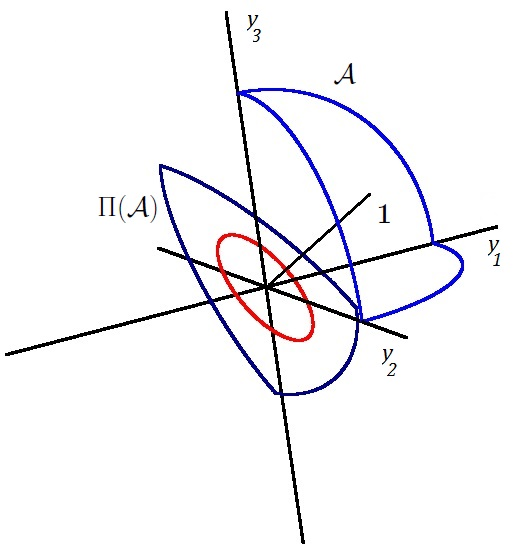
\includegraphics[width=4in]{minSS3dSampleSpace.jpg}
%\caption{A depiction of $\mathcal{A}$, $\Pi(\mathcal{A})$, and the
%  unit circle for the illustrative example where $b_{1}(\mathbf{1},\by)=\min(\by)=0$ and
%  $s(\mathbf{1},\by)=\sum (y_i -b_{1}(\mathbf{1},\by))^2 =1$.
%$\mathcal{A}$ is the combination of three quarter circles, one
%  on each plane defined by $y_i=0$. The projection of this manifold
%  onto the deviation space is depicted by the bowed triangular shape
%  in the plane defined by $\sum y_i=0$. The circle in this plane
%  represents the sample space for the intermediate sample \green{$\bz^*$}. Also
%  depicted is the vector $\mathbf{1}$, the design matrix for the
%  location and scale setting.}
%\label{fig:sampSpace}
%\end{figure}

The set $\mathcal{A}$ typically does not lie in a linear space of dimension $n - p - 1$, and 
so we must account for both the many-to-one nature of the mapping and
a Jacobian when deriving the proposal density.  We handle the first
point by sampling the initial $\bz^*$ from
 a reduced $n - p - 1$ dimensional space which, through the scaling and
shifting of the above theorem, maps uniquely to a point 
in $\mathcal{A}$. This reduced space is chosen so that the range of the map is the
entirety of $\mathcal{A}$.  The Jacobian does not cancel in
\eqref{MHRatio}, since the scaling depends on the initial proposal. 

The reduced space from which the initial sample is taken is simply the
unit sphere \green{\sout{restricted to} in} the orthogonal complement of the column space of the design matrix (i.e., the least squares residual space). To help understand the density of the proposal derived from the transformation of this initial sample we introduce the following notation. Denote the column space of the design matrix $X$ by $\mathcal{C}(X)$ and its orthogonal complement by $\mc{C}^\perp(X)$. 
\green{\sout{This} The latter} is the least squares residual space which we will often refer to as the `deviation space'.  The projection of the set $\mathcal{A}$ onto the deviation space is 
\begin{equation}
\label{sampleSpacePerp}
\Pi(\mathcal{A})=\{\bz\in \mathbb{R}^n |\ \exists\ \by\in \mathcal{A}\
s.t.\ \bz=Q \by \}
\end{equation} 
where $Q$ is the projection matrix onto  $\mc{C}^\perp(X)$. Explicitly, $Q=I-H$ with $H=XX^\top$ where we assume, without
loss of generality following condition \ref{fullRank},  that the
columns of $X$ form an orthonormal basis for $\mc{C}(X)$
(i.e., $X^\top X=I$). It will also be helpful at times to write $Q=WW^{\top}$ where the columns of $W$ form an orthonormal basis for $\mc{C}^\perp(X)$. This set has been introduced because we will first transform the initial distribution on the sphere to the distribution on this set. Then we will transform to the \green{\sout{sample space} set} $\mc A$.

Returning to the artificial example, Figure~\ref{fig:sampSpace}
depicts $\Pi(\mathcal{A})$ as well as the sphere from which we obtain
the initial sample. The column vector $X=\bf{1}$ spans $\mc{C}(X)$ and
is shown as a reference. The triangle with bowed sides in dark
  blue is  $\Pi(\mathcal{A})$, the projection of $\mc A$ onto the
plane orthogonal to $\mb 1$ (i.e., $\mc{C}^\perp(X)$). The \green{unit} sphere from
which the initial sample is taken is depicted as the red circle in this plane.  In general, this is the unit sphere in the $n-p$ dimensional space $\mc{C}^\perp(X)$.  

For the transformation of the initial proposal $\bz^*$ on the surface of the sphere to $\by\in \mc A$ , we first move to a point on $\Pi(\mathcal{A})$ through a 
simple scaling of $\bz^*$.  This is followed by undoing the projection with a move from 
$\Pi(\mathcal{A})$ to its (unique) preimage on $\mathcal{A}$. Together, these two steps correspond to the
transformation in Theorem~\ref{Transformation}.  The introduction of
the sphere in $\mc {C}^\perp (X)$ as the initial proposal surface
along with properties \ref{regEq}-\ref{scaleEq2Reg} ensure that the mapping is
1-1. In particular, property
\ref{scaleEq2Reg} ensures the scaling to be unique and \ref{regIn}
implies that the scale statistic is unchanged when undoing the
projection. Property \ref{regEq} ensures the uniqueness of undoing the
projection.  The general proposal strategy is summarized as follows:
\begin{enumerate}
\item Sample $\bz^*$ from a distribution with known density on the unit sphere in $\mc{C}^\perp(X)$.
\item Calculate the Jacobian of \green{the} transformation in Theorem \ref{Transformation} in two steps.
\begin{enumerate}
\item Scale from unit sphere to $\Pi(\mathcal{A})$: $\bz=\frac{s(X,\boldsymbol{y}_{obs})}{s(X, \boldsymbol{z}^{*})}\bz^{*}$
\item Shift  from $\Pi(\mathcal{A})$ to $\mathcal{A}$: $\by=\bz+X\left(\bb(X, \by_{obs})-\bb(X, \bz)\right)$
\end{enumerate}
\end{enumerate}

\subsubsection{Evaluation of the proposal density} 
Calculation of the appropriate Jacobian of the transformation is absolutely vital and also non-trivial. Writing the transformation from the unit sphere in deviation space to $\mathcal{A}$ in 
two steps facilitates calculation of the Jacobian in two steps as written above. % \textcolor{blue}{added the following sentence, hopefully it helps}
We now explain each step, keeping in mind that the Jacobian of a transformation is simply the ratio of infinitesimal volumes along the tangents of the domain and range of the transformation. 

\vskip 0.05 in
\noindent
{\bf Scale from unit sphere to $\Pi(\mathcal{A})$} \\
The first step is constrained to $\mc{C}^\perp(X)$ where the unit sphere is transformed to $\Pi(\mathcal{A})$. We further break this \green{\sout{piece} step into \sout{in two steps} into two substeps}: first, the distribution on the unit sphere is transformed to that along a sphere of radius $r=\|\bz\|={s(X,\boldsymbol{y}_{obs})}/{s(X, \boldsymbol{z}^{*})}$. This contributes \green{a factor of} $r^{-(n-p-1)}$ to the Jacobian. Second, the new sphere is then deformed to $\Pi(\mathcal{A})$.  This deformation contributes an attenuation to the Jacobian equal to the
ratio of infinitesimal volumes in the
tangent spaces of the sphere and $\Pi(\mathcal{A})$ at $\bz$.  
Restricting ourselves to the $n-p$ dimensional space $\mc{C}^\perp(X)$, this
ratio is the cosine of the angle between the normal 
vectors of the two sets at $\bz$.  The normal to the sphere is its radius vector $\bz$. The normal to
$\Pi(\mathcal{A})$ is given in the following lemma.  

\begin{lemma}
\label{gradSTheoremReg}
Assume that conditions \ref{fullRank}-\ref{supReal}, \ref{as}, and \ref{regIn} hold.  
Let $\by\in \mathcal{A}$. Let 
$\nabla s(X,\by)$ denote the
gradient of the scale statistic with respect to the data vector evaluated at
$\by$.  Then $\nabla s(X,\by)\in \mc{C}^\perp(X)$ and is 
normal to $\Pi(\mathcal{A})$ at $\bz=Q\by$  in $\mc{C}^\perp(X)$.
\end{lemma}

As a result of the lemma, the contribution to the  Jacobian of this attenuation is 
\begin{equation}
\label{cosine}
\cos(\gamma)=\frac{\nabla s(X,\by)^\top \bz}{\|\nabla
s(X,\by)\| \|\bz\|},
\end{equation}
where $\gamma$ is the angle between the two normal vectors.
This step is illustrated in Figure~\ref{fig:stretchDeform} for the toy
location-scale example.  The figure \green{\sout{only}} pictures \green{only} the deviation space
which in this case is a plane. The original unit  sphere (here, the
solid circle) is first stretched to the dashed sphere contributing
$r^{-(n-p-1)}$ to the Jacobian as seen in panel (a). In panel (b), the
dashed circle is transformed onto $\Pi(\mc A)$ contributing
$\cos(\gamma)$ to the Jacobian. The normal vectors in panel (b) are
orthogonal to the tangent vectors of $\Pi(\mc A)$ and the circle. As
stated above, the Jacobian is the ratio of infinitesimal lengths along these tangent vectors. This is the same as the ratio of the infinitesimal lengths of the normal vectors (i.e., $\cos(\gamma)$). This generalization extends to higher dimensions where the `lengths' along the tangent vectors become volumes along the tangent spaces. 

%\begin{sidewaysfigure}[t]
%\centering
%\captionsetup{justification=centering}
%\subcaptionbox{}{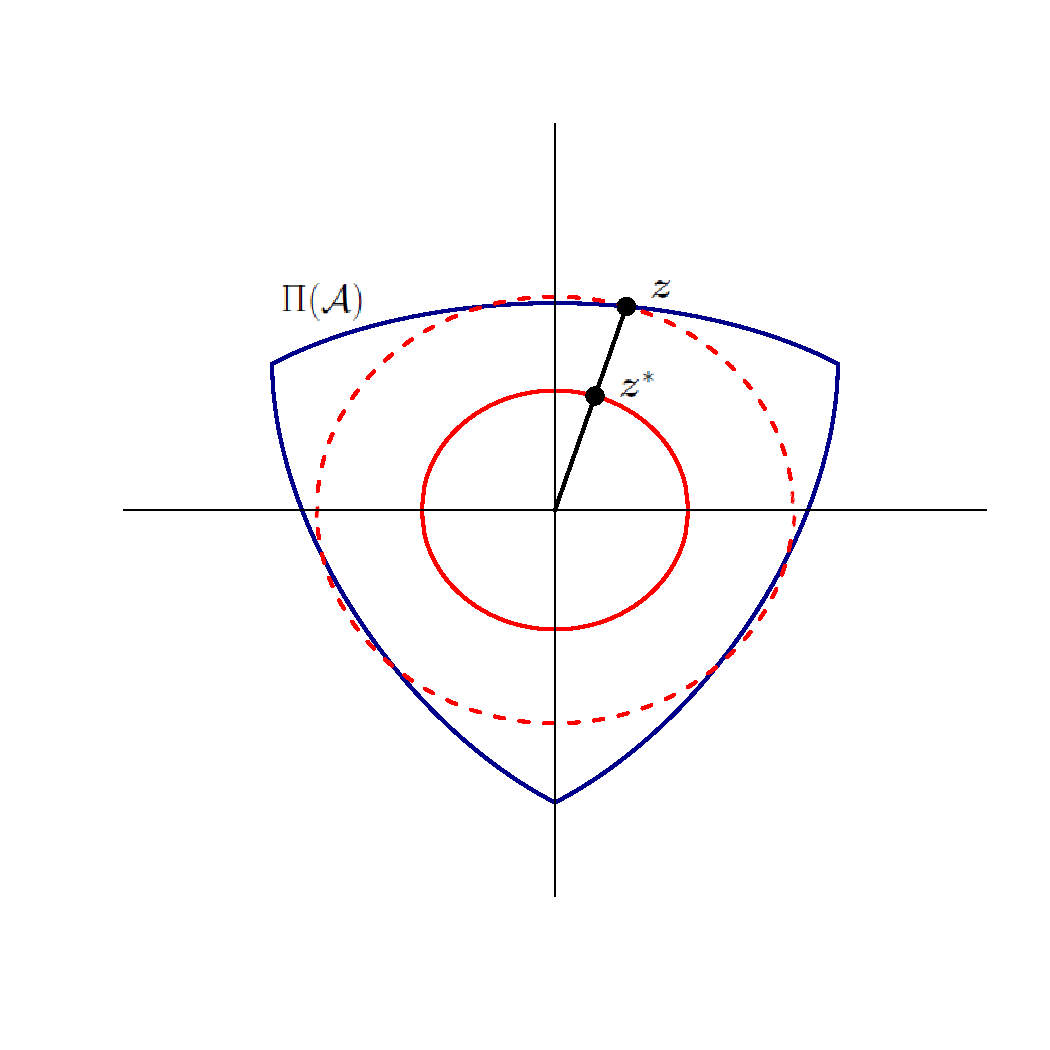
\includegraphics[width=4in]{minSSZSpace3.pdf}}\quad
%\subcaptionbox{}{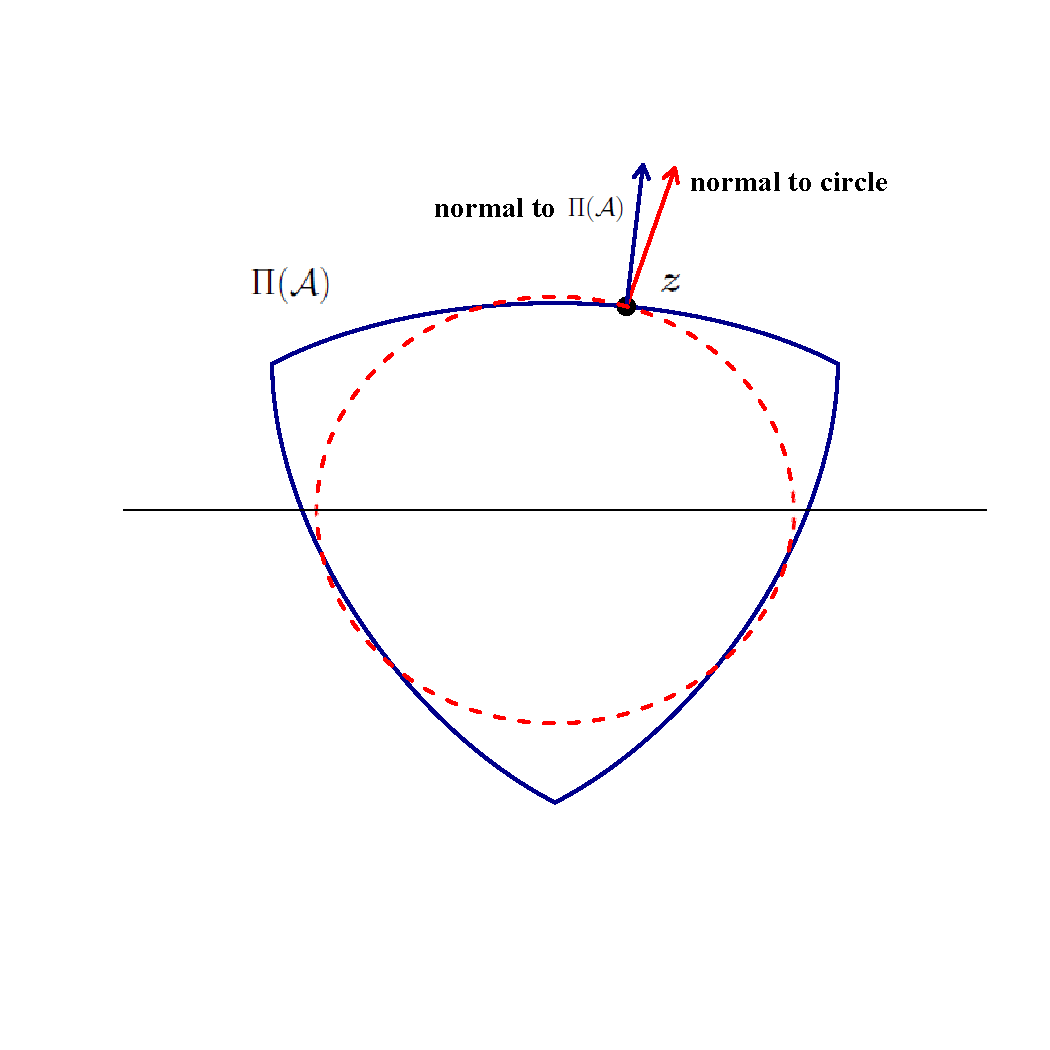
\includegraphics[width=4in]{minSSZSpace5.pdf}}
%\caption{Panel (a) contains a depiction of the stretch from $\bz^{*}$
%  to $\bz$. The adjustment for the stretch transforms the density
%  along the unit circle to the density along the circle of radius
%  $\|\bz\|$ (dashed circle).  Panel (b) contains a depiction of the
%  deformation from the distribution along the circle to the
%  distribution along $\Pi(\mathcal{A})$. The adjustment can be seen to
%  be the cosine of the angle between the normals to each manifold.}
%\label{fig:stretchDeform}
%\end{sidewaysfigure}

\vskip 0.05 in
\noindent
{\bf Shift from $\Pi(\mathcal{A})$ to $\mathcal{A}$} \\
The final piece of the Jacobian comes from the transformation from
$\Pi(\mathcal{A})$ to $\mathcal{A}$.  %For this we return to the full $n$ dimensional space.  
This step involves a shift of
$\bz$ to $\by$ along the column space of $X$. Since the shift depends on 
$\bz$, the density on the set 
$\Pi(\mathcal{A})$ is deformed by the shift. The
contribution of this deformation to the Jacobian is, again,
the ratio of the infinitesimal volume along $\Pi(\mathcal{A})$ at $\bz$ to the
corresponding volume along $\mathcal{A}$ at $\by$. 
The ratio is calculated by considering the volume of the
projection of a unit hypercube in the tangent space of $\mathcal{A}$
at $\by$ onto $\mc{C}^\perp(X)$.
Computational details are
given in the following lemmas and subsequent theorem. Throughout, let
$\mc T_{y}(\mc A)$ and $\mc T_{y}^{\perp}(\mc A)$ denote the tangent
space to $\mc A$ at $\by$ and its orthogonal complement respectively. 

\begin{lemma}
\label{lem:basis}
Assume that conditions \ref{fullRank}-\ref{regEq} and \ref{regIn}-\ref{scaleEq2Reg} hold.  Then the $p+1$ gradient vectors 
$\nabla s(X,\by), \nabla b_1(X,\by),\dots, \nabla b_p(X,\by)$ form a
basis for $\mc T_{y}^\perp(\mc A)$ with probability one.
\end{lemma}

The lemma describes construction of a basis for $\mc T_{y}^\perp(\mc A)$.  This leads to a 
basis for $\mc T_{y}(\mc A)$.  Both of these bases can be orthonormalized.  
Let $A=[a_{1},\dots,a_{n-p-1}]$  and $B=[b_1,\dots,b_{p+1}]$ denote the 
matrices whose columns contain the orthonormal bases for  $\mc T_{y}(\mc A)$ and  $\mc T^{\perp}_{y}(\mc A)$, respectively.  
The columns in $A$ define a unit hypercube in $\mc T_{y}(\mc
  A)$ and their projections onto $\mc{C}^\perp(X)$ define a parallelepiped.
We defer construction of $A$ until later. 

\begin{lemma}
\label{lem:fullrank}
Assume that conditions \ref{fullRank}-\ref{regEq} and \ref{regIn}-\ref{scaleEq2Reg} hold.  
Then the $n\times (n-p-1)$ dimensional matrix $P=QA$ is of full column rank.
\end{lemma}

As a consequence of this lemma, 
the parallelepiped spanned by the columns of $P$ is not
degenerate (it is $n-p-1$ dimensional), and its volume
is given by
\begin{equation}
\label{eq:volume}
\text{Vol} (P) := \sqrt{\text{det}(P^\top P)}=\prod_{i=1}^{r} \sigma_i
\end{equation}
where $r=\text{rank} (P)=n-p-1$ and $\sigma_1\geq
\sigma_2\geq\dots\geq\sigma_r>0$ are the singular values of $P$ (e.g.,
\cite{miao1992}). 
Combining Lemmas \ref{lem:basis} and \ref{lem:fullrank} above leaves us with the following result concerning the calculation of the desired Jacobian.  
\begin{theorem}
\label{Jacobian}
Assume that conditions \ref{fullRank}-\ref{regEq} and \ref{regIn}-\ref{scaleEq2Reg} hold.  Then the
Jacobian of the transformation from the distribution along 
$\Pi(\mc A)$ to that along $\mc A $ is equal to the volume given in \eqref{eq:volume}.
\end{theorem}

\vskip 0.05 in
\noindent
{\bf The proposal density} \\
Putting all the pieces of the Jacobian together we have the following result. Any dependence on other variables, including current states in the Markov chain, is made implicit. 
\begin{theorem} 
Assume that conditions \ref{fullRank}-\ref{scaleEq2Reg} hold.  Let $\bz^{*}$ be sampled on the unit sphere in $\mc {C}^\perp (X)$ with density $p(\bz^{*})$.  Using the transformation of $\bz^*$ to $\by\in \mc A$ described in Theorem \ref{Transformation}, the density of $\by$ is
\begin{equation}
\label{dens:ystst}
p(\by)=p(\bz^*) r^{-(n-p-1)} \cos(\gamma)\text{Vol} (P)
\end{equation}
where $r={s(X,\boldsymbol{y}_{obs})}/{s(X,  \boldsymbol{z}^{*})}$,
and $\cos(\gamma)$ and $\text{Vol} (P)$ are as in equations \eqref{cosine} and \eqref{eq:volume}, respectively. 
\end{theorem} 

In practice, computing $A$ directly to find $P$ and $\text{Vol} (P)$ is computationally intensive as it involves orthogonalization of $n$ vectors in $n$-dimensional space. 
To find a matrix $A$, supplement $B$ with a set of $n$ linearly independent columns on the right, and apply Gram-Schmidt 
orthonormalization to the matrix.  This algorithm is infeasibly slow when $n$ is large because it is $\mc O(n^3)$ and must be repeated at each
iterate of the MCMC when a complete data set is drawn.  
Fortunately, we can make use of results related to \textit{principal angles} found in \cite{miao1992} to compute the volume in \eqref{eq:volume} using $B$ and an orthonormal basis for $\mc C (X)$ (The definition of principal angles can be found in the cited text). Recall, $B$ is constructed by orthogonalization of a basis for $\mc T_{y}^\perp(\mc A)$. Since this space is of dimension $p+1$, applying Gram-Schmidt to find the orthonormal basis is much faster, the algorithm is $\mc O(np^2)$, and there is a 
considerable reduction in computational burden when $n \gg p$. 
Further, the singular values of $P=QA$ are also the singular values of
$W^\top A$ (recall, $Q=WW^{\top}$), which can be easily obtained through $B$.
The following corollary formally states how computation of $A$ can be circumvented. 
\begin{corollary}
\label{theorem:sings}
Let $U$ be a matrix whose columns
form an orthonormal basis for $\mc C (X)$. Then the non-unit singular
values of $U^\top B$ are the same as the non-unit singular values of $W^\top A$.  
\end{corollary} 
\noindent Thus, we can compute $\text{Vol} (P)$ by finding the singular values of $U^\top B$, reducing the computational burden substantially. 

%%%%%%%%%%%%%%%%%%%%%%%%%%%%%%%%%%%%%%%%%%%%%%%%%%%%%%%%%%%%
%
% Applications
%
%%%%%%%%%%%%%%%%%%%%%%%%%%%%%%%%%%%%%%%%%%%%%%%%%%%%%%%%%%%%
\section{Applications}
\label{Applications}
We illustrate the methods developed in Sections~\ref{restrictedlikelihood} and \ref{BayesLinMod} with a pair of regression models for 
data from Nationwide Insurance Company, which concern prediction of
the performance of insurance agencies.
The data contain outliers and are subject to model misspecification.  
In particular, a group of the data do not follow the same generative process as the data of interest.  It would be 
extremely challenging to model some features of the data.  
In our analysis, we follow the standard practice when demonstrating the benefits of robust 
methods.  We work with a naive model for the data which ignores certain features of the problem.  We
do this both to create a situation where all can agree that the model for the full data $\by$ is imperfect
and to preserve the confidentiality of selected aspects of modelling done by Nationwide.  
We wish to provide inference for the `good' portion of the data.  The two models we fit either treat the analysis
as a single regression or as a collection of related regressions.  Details of the models, prior distributions, 
and conditioning statistics are given in the next two subsections.  

%%%%%%%%%%%%%%%%%%%%%%%
%NW data
%%%%%%%%%%%%%%%%%%%%%%%

\subsection{Nationwide Data}
The Nationwide Insurance Company sells many of its insurance policies through agencies which provide direct service to policy holders.  
The contractual agreements between Nationwide and these agencies vary.  Of major interest to Nationwide is the prediction of future performance of agencies where, for our purposes,  performance is measured by the total number of households an agency services (`household count'). A serviced household is one in which at least one person living at that residence has at least one policy written through the agency. We used data from previous years to build a model to forecast future household count. In particular, we use agency characteristics, as measured during a single month in $2010$, to predict household counts in the corresponding month in $2012$. The characteristics used are household count and two measurements of agency size/experience. The two measurements of agency size/experience are, roughly, the number of employed persons at the agency and the length of time the agency has been affiliated with Nationwide. The household counts (response and predictor) have been square rooted to stabilize variance. The data are 
proprietary, and to mask them all variables have been individually centered and scaled and identifiers (agency/agent names and state
labels) have been removed. 
All subsequent analysis is done on this scale.  As an exploratory view, a plot of the square root of count in 2012, against that in 2010 
is shown in Figure \ref{fig:ctVct}.  The different colors represent the varying contractual agreements as they stood in 2010. `Type 1' agencies are of special interest.  Among the open agencies, a strong linear correlation exists.  The specific linear relationship
depends on agency type. The data are characterized by a large number of agencies which were open in 2010 but closed sometime before 2012, as represented by the horizontal band at $0$. We use these data as a test bed for our techniques, fitting models that do not account for agency closures or contract type.  Our expectation is that \green{\sout{the incomplete} restricting the} likelihood will facilitate prediction for the good part of the data.  

%\begin{figure}[t]
%\centering
%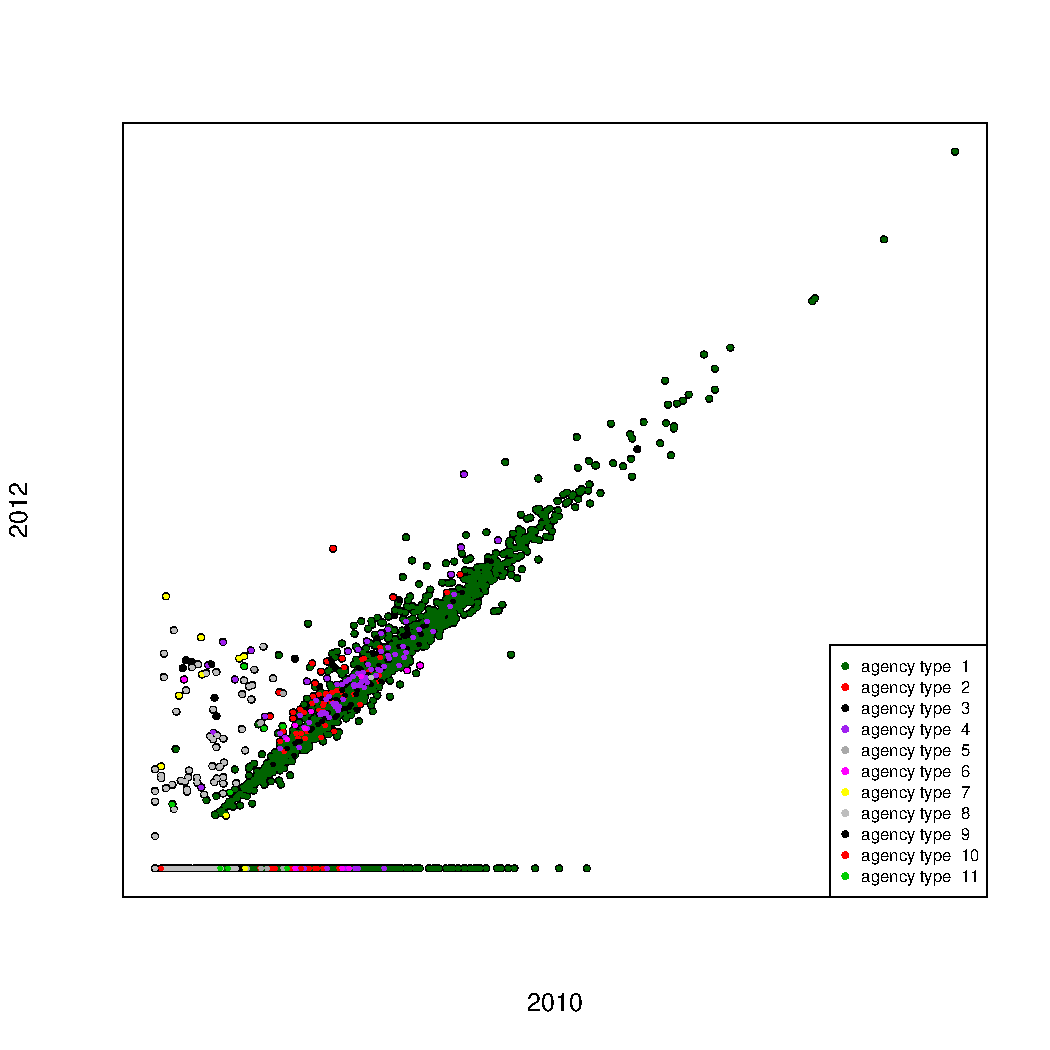
\includegraphics[width=4in]{countvcount.pdf}
%\caption{The square root of count in 2012 versus that in 2010 (after centering and scaling). The colors represent the varying contractual agreements as they stood in 2010.  Agencies that closed during the 2010-2012 period are represented by the zero counts for 2012. Scalings on the axes are purposely left off for proprietary reasons.}
%\label{fig:ctVct}
%\end{figure}

\subsection{Regression model}
\label{regModelNW}
The first analysis that we consider is based on a single regression.  We use 
the following standard normal theory regression model 
\begin{equation}
\label{eq:regModel}
\bbeta\sim N_p(\bmu_0, \Sigma_0);\ \ \sigma^2\sim IG(a_0,b_0);\ \  
y_{i}=\bx_{i}^\top\bbeta+\epsilon_{i},\ \ \epsilon_{i}\iid N(0, \sigma^2),\ i=1,\dots, n, 
\end{equation}
where $\bbeta$ is a four dimensional vector ($p=4$) of regression coefficients for the intercept, square root of count in 2010, and the two size/experience measures, and $y_{i}$ is the square rooted household count in 2012 for the $i^{th}$ agency with covariate vector $\bx_{i}$.  Although the mean of covariates and response have been removed, we include the intercept as fitting is done on a holdout set to evaluate predictive performance.  
The hyper-parameters $a_0, b_0, \bmu_0$ and $\Sigma_0$ are all fixed and set from a 
robust regression fit to the data from the time period two years
before. Letting $\hat\bbeta$ represent the estimate of the coefficients from this fit we  set $\bmu_0=\hat\bbeta$ and $ \Sigma_0=n\cdot \mbox{var}(\hat\bbeta)$ where here $n$ is the sample size of the prior data set.  %corresponding to  a unit information prior for $\bbeta$. 
The hyperparameters for $\sigma^2$ are set so that the prior mean is $s^2$, the estimated variance from the robust regression, and the spread of the prior covers the range of plausible values with high probability. All values are then transformed appropriately to match the current scale of the data. In the end we take $\bmu_0=(0.18,  0.81,0.01,-0.02)^\top$ and set the mean of $\sigma^2$ to $0.014$ and standard deviation to  $0.033$. 

We compare four Bayesian models: the standard Bayesian normal theory model, two restricted likelihood models, both with simultaneous M-estimators, and a heavy-tailed model.  For the restricted likelihood methods we use the same simultaneous M-estimators as in Section \ref{darwinAnalysis} adapted to linear regression.  The heavy-tailed model replaces the normal sampling density in \eqref{eq:regModel} with a $t$-distribution with $\nu = 3$ degrees of freedom. %We have used the default tuning parameter settings for the {\tt rlm} function in the R package {\tt MASS} \citep{venables2002}.  Both use Huber's scale estimator as in the {\tt rlm} implementation.  
We also fit the corresponding classical robust regressions and a least squares regression.  

\subsubsection{Method of model comparison}
We wish to examine the performance of the models in a fashion that preserves the essential features of the 
problem.  Since we are concerned with outliers and model 
misspecification, we understand that our models are imperfect and so prefer to use an out-of-sample measure of fit.  
This leads us to cross-validation.  We repeatedly split the data into training
and validation sets.  We fit the model to the training data and assess its performance on the validation data.  

The presence of numerous outliers in the data implies that both training and validation data will contain 
outliers.  For this reason, the evaluation must be robust to a certain fraction of bad data.  
The two main strategies are to robustify the evaluation function \citep[e.g.,][]{ronchetti1997} or 
to retain the desired evaluation function and trim cases \citep{jung2014}.  Here,
we pursue the trimming approach with log predictive density for the Bayesian models and log plug-in 
maximum likelihood for the classical fits used as the evaluation function.

The trimmed evaluation proceeds as follows in our context.  The evaluation function for case $i$ in the hold-out data
is the log predictive density, say
$\log(f(y_i))$, with the conditioning on the 
summary statistic suppressed.  The trimming 
fraction is set at $0 \leq \alpha < 1$. To score a method,
we first identify a base method. Denote the predictive density under this method by $f_{b}(y)$.  Under the base method, $\log(f_{b}(y_i))$ is computed for each case in the 
validation sample, say $i = 1, \ldots, M$.  Order the validation
sample according to the ordering of $\log(f_{b}(y_i))$ and denote this
ordering by $y_{(1)}^b, y_{(2)}^b, \dots, y_{(M)}^b$. That is, for $i<j$
$\log(f_{b}(y_{(i)}^b))<\log(f_{b}(y_{(j)}^b))$. All of the methods are then scored on the validation sample with the mean trimmed log marginal pseudo likelihood, 
\[TLM_b(A) = (M - [\alpha M])^{-1} \sum_{i=[\alpha M]+1}^{M}
    \log(f_A(y_{(i)}^b)),\]
 where $f_A$ corresponds to the predictive
 distribution under the method ``A'' being scored.  In other words, the $[\alpha M]$ observations with the smallest values of $\log(f_{b}(y))$ are 
removed from the validation sample and all of the methods are scored using only the
remaining $M - [\alpha M]$ observations. This process is advantageous to the base method.  A method
that performs poorly when it is the base method is discredited.  For a complete evaluation, we allow each method
to appear as the base method.  For brevity, we present only a selection of results in our subsequent analyses.  

\subsubsection{Comparison of predictive performance}
Model performance is assessed
using the mean and standard deviation of the TLM 
across $100$ different splits into training and validation samples. First, we include all observations
in each validation sample to calculate TLM for each split. We then
repeat the evaluation using only certain subsets of the validation
sample that are of special interest. Subsets include open agencies,
open `Type 1' agencies, and `Type 1' agencies. For brevity, we include
results for the `Type 1' agencies only. As noted, assessing model
predictions on this set of agencies is of special interest to the
company.  A range of training sample sizes was used and we include
results from $n=25,100,1000,$ and $2000$ out of a total of $3180$ agencies. The trimming fraction, $\alpha$, ranges from $0$ to $0.3$. A classical robust regression to the prior data assigns zero weight to around $16\%$ of observations; in essence removing these from the analysis. This informed the range of trimming fractions chosen.  
In practice, we would set $\alpha$ slightly larger than $0.16$.  


%\begin{sidewaysfigure}
%\centering
%\captionsetup{justification=centering}
%%\subcaptionbox{}{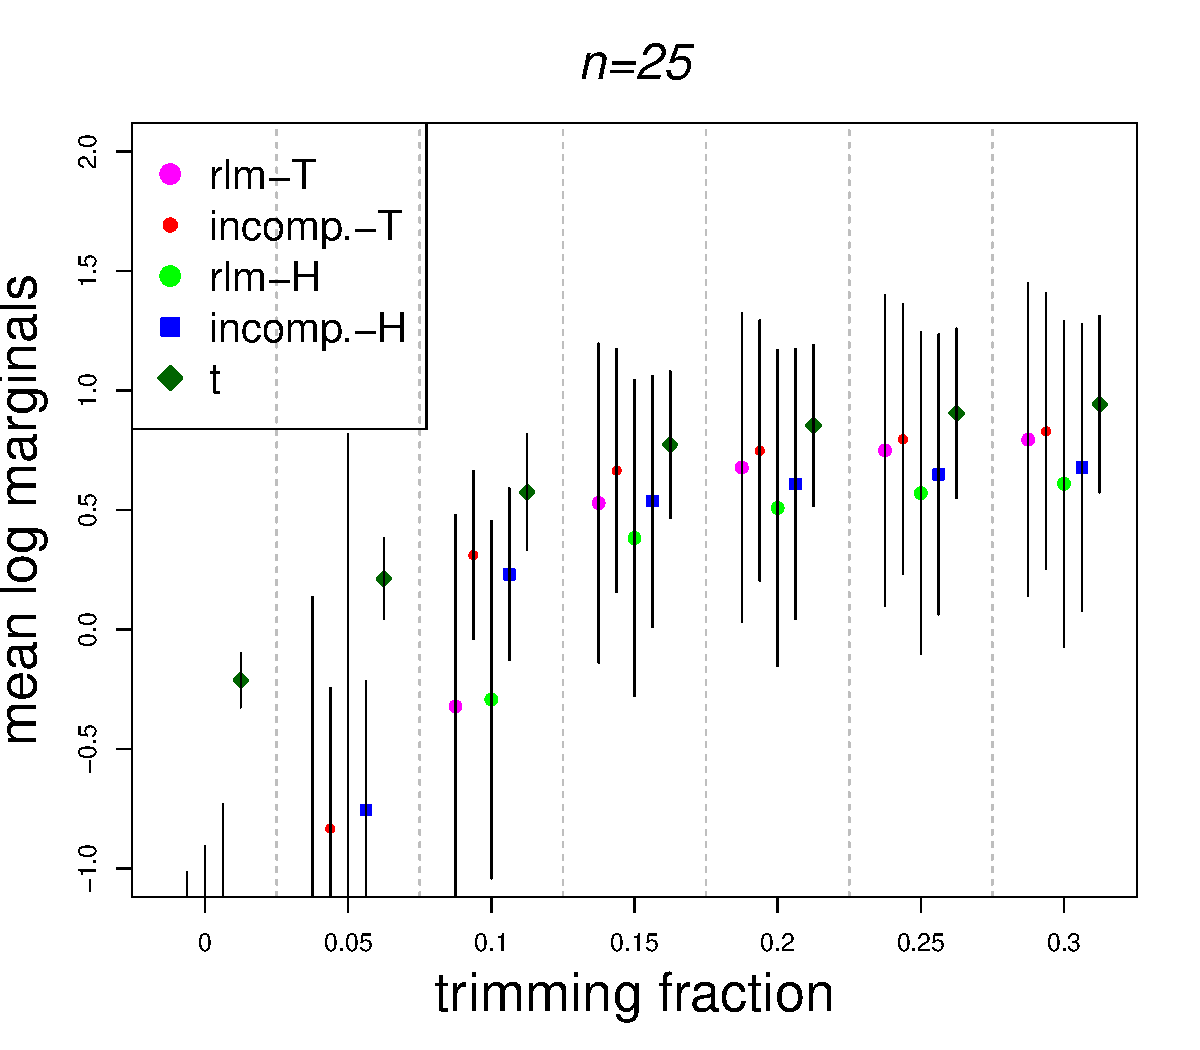
\includegraphics[width=\textwidth,page=1]{logMargType1AgenciesBaseModelt}}\quad
%%\subcaptionbox{}{\includegraphics[width=\textwidth,page=2]{logMargType1AgenciesBaseModelt}}\quad
%%\subcaptionbox{}{\includegraphics[width=\textwidth,page=3]{logMargType1AgenciesBaseModelt}}
%\subcaptionbox{}{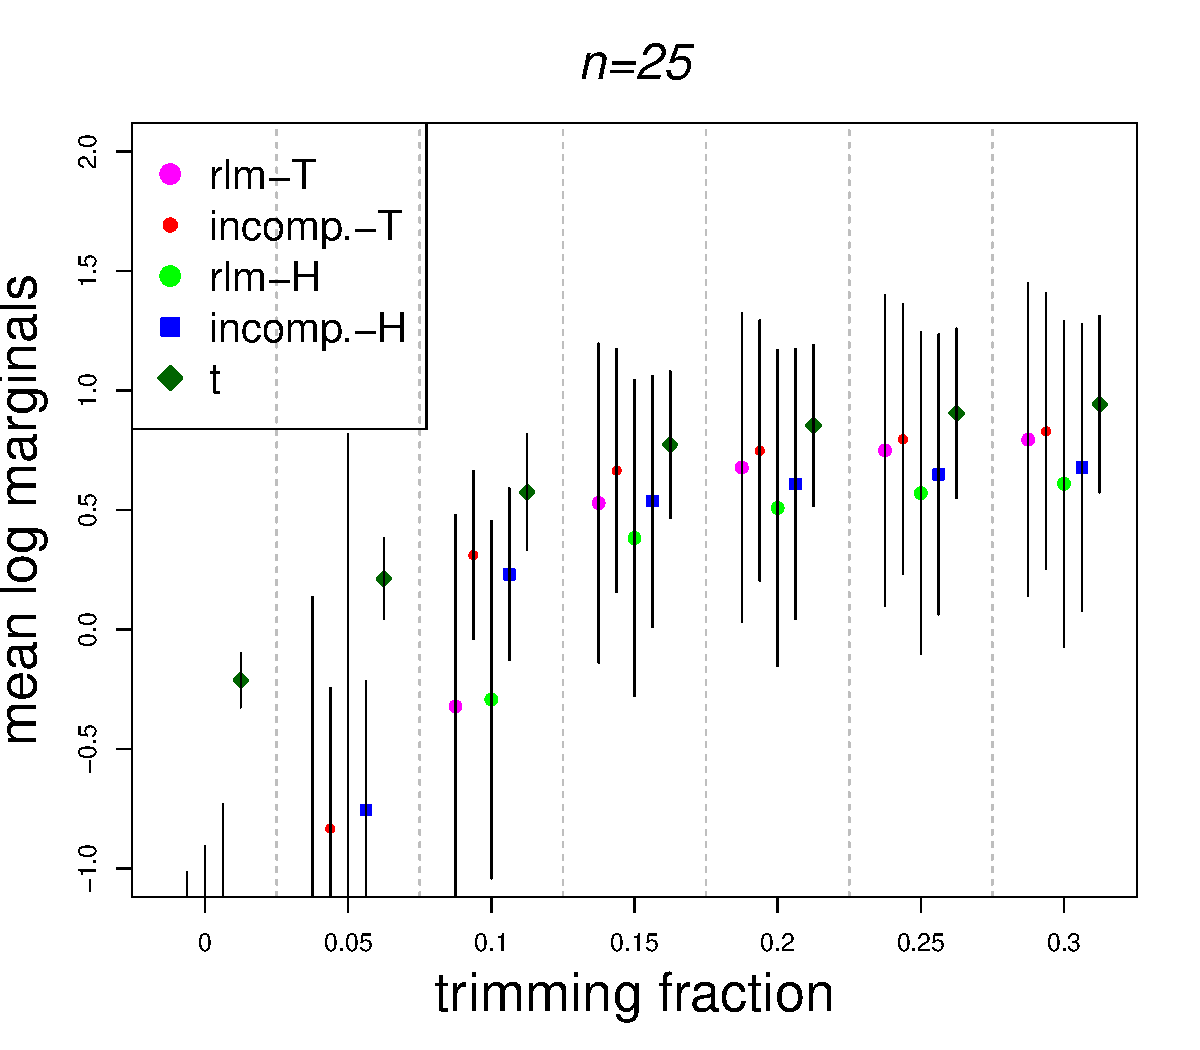
\includegraphics[width=3.4in,height=3.3in, page=1]{logMargType1AgenciesBaseModelt}}\quad
%\subcaptionbox{}{\includegraphics[width=3.4in,height=3.3in,page=2]{logMargType1AgenciesBaseModelt}}\quad
%\subcaptionbox{}{\includegraphics[width=3.4in,height=3.3in,page=3]{logMargType1AgenciesBaseModelt}}
%\caption{Model evaluation for `Type 1' agencies for training sample
%  sizes of $n=25,100$, and $1000$. The $t$-model is used as the base
%  method to compute TLM. Plotted are the mean TLM for each model
%  against the trimming fraction across the $100$ cross-validation
%  samples. Error bars correspond to one standard deviation of TLM
%  above and below the mean. Models are labeled with the following
%  abbreviations: `rlm' corresponds to a classical robust fit, `restr.'
%  corresponds to our restricted likelihood method, and `t' corresponds to the
%  heavy-tailed $t$-distribution model. The letters `T' and `H'
%  appearing after `rlm' and `restr.' correspond to the use of  Tukey's
%  and Huber's $\psi$ respectively.  
%}
%\label{fig:Type1Marg}
%\end{sidewaysfigure}
%


Model evaluation for `Type 1' agencies is shown in Figure
\ref{fig:Type1Marg} for training sample sizes $n=25, 100,$ and $1000$.
The $t$-model is used as the base
  method to compute TLM.
The models pictured are: classical robust regression with Tukey's $\psi$ function (rlm-T), restricted likelihood with Tukey $\psi$ (restr.-T), classical robust regression with Huber's $\psi$ function (rlm-H), restricted likelihood  with Huber's $\psi$ (restr.-H), and the thick tailed $t$-model (t). The normal theory models perform poorly due to the numerous outliers
and are left out of the figures. Appearing in the figures are the mean TLM across
validations set for each model and each trimming fraction, $\alpha$ (along the $x$-axis). The error bars depicted are one standard deviation of the TLM above and below the mean.  The range of the vertical axis is chosen to enhance important features and as a result, some evaluation measures extend below this range. In particular, the restricted likelihood methods perform poorly if no trimming is done; reflecting that these methods are not intended to fit well to outliers. Recall that we expect about 15-16\% outliers in the validation sets, thus trimming fractions slightly larger than this amount are needed in order to assess fits to the `good' data. For $n=25$, the thick tailed model  prevails across trimming fractions, although less so for $\alpha\geq 0.15$. For sample sizes as low as $n=100$, the restricted likelihood methods outperform the heavy-tailed model with the Tukey version performing the best.   
The stronger performance of restricted likelihood based on Tukey's method and the t model is to be expected, as many of the 
residuals are so extreme that trimming is better than winsorizing (as Huber's method effectively does).  
As expected, with enough data,  the Bayesian methods and their classical counterparts perform similarly, although there
is a persistent slight edge in favor of the Bayesian restricted likelihood methods.  We attribute this advantage to the weakly informative
prior distribution which pulls the estimates slightly toward better values.  The similarity occurs as early as $n=100$. 

 
\subsection{Hierarchical regression model}
\label{hierRegNW}
Nationwide agencies span many states and insurance regulations and the competitive environment varies between states. A natural extension to the previous analysis is a hierarchical regression model, grouping agencies within each state to reflect similar business environments. Using the same study design with the same training and validation splits, we re-analyze the data using the following hierarchical regression model:
\begin{align}
%\begin{split}
\label{eq:hierModel}
&\bbeta\sim N_p(\bmu_0, a\Sigma_0);\ \ 
\bbeta_j\iid N_p(\bbeta, b\Sigma_0); \ \  
\sigma_j^2\sim IG(a_0,b_0);  & \\ \nonumber
& \by_{ij}=\bx_{ij}^\top\bbeta_j+\epsilon_{ij},\ \ \epsilon_{ij}\iid N(0, \sigma_j^2),\ i=1,\dots, n_j,\ j=1,\dots, J &
%\end{split}
\end{align}
where $y_{ij}$  represents the $i^{th}$ observation in the $j^{th}$
state, $n_j$ is the total number of agencies in each state, and $J$ is
the number of states. $\bx_{ij}$ is a four dimensional vector
comprised of the same covariates as above. $\bbeta_j$ represents the
individual regression coefficient vector for state $j$.  We match this
model to the non-hierarchical model in several ways. First, $\bmu_0$,
$\Sigma_0$, $a_0$, and $b_0$ are fixed as before. We constrain $a+b=1$
in an attempt to partition the total variance between the individual
$\bbeta_j$'s and the overall $\bbeta$. We take $b\sim
\text{beta}(v_1,v_2)$. Using the previous data set, we assess the
variation between individual estimates of the $\beta_j$ to set $v_1$
and $v_2$ to allow for a reasonable amount of shrinkage. To allow for
dependence across the $\sigma_j^2$ we first take
$(z_1,\dots,z_J)\sim N_J(\mathbf{0}, \Sigma_\rho)$ with
$\Sigma_\rho=(1-\rho)I+\rho \mb{1}\mb{1}^{\top}$. Then we set
$\sigma^2_j=H^{-1}(\Phi(z_j))$ where $H$ is the cdf of an
$IG(a_0,b_0)$ and $\Phi$ is the cdf of a standard normal. This results in the specified marginal distribution, while
introducing correlation via $\rho$. We assume $\rho\sim
\text{beta}(a_\rho,b_\rho)$ with mean $\mu_\rho=a_\rho/(a_\rho+b_\rho)$ and precision
$\psi_\rho=a_\rho+b_\rho$. The parameters $\mu_\rho$ and
$\psi_{\rho}$  are given beta and gamma distributions, respectively. We fix the parameters of these distributions by again considering fits to individual states from the previous data set. More precise details on setting $v_{1}, v_{2}$ and the the priors on $\mu_{\rho}$ and $\psi_{\rho}$ are given in the appendix. We note that we tried a range of other fixed hyper-parameters resulting in negligible differences in the results. 

Using the same techniques as in the previous section, 
we fit the normal theory hierarchical model above, a thick tailed $t$ version with $\nu = 3$ d.f., and two restricted likelihood versions (Huber's and Tukey's) of the model.  For the incomplete restricted methods, we condition on robust regression estimates fit separately within each state. We also fit classical robust regression counterparts and a least squares regression separately within each state.  

We digress briefly to note that for the restricted likelihood methods no additional computational strategies outside of those discussed in Section~\ref{highDim} are needed to fit the hierarchical models described here. Since we condition on statistics which are computed within each state, the model's conditional independence between the states allows the data augmentation described earlier to be performed independently within each state.  Updates of hyperparameters follow conventional MCMC procedures.  We note that different types of statistics could be chosen for each state, if desired, allowing for a large amount of flexibility.  

Selected results for the hierarchical fits appear in Figure
\ref{fig:hierType1Marg}. Hierarchical models naturally require more
data and so we consider only training sizes of $n=1000$ and
$2000$.  Again, the $t$-model is used as the base
method for computing TLM. Trimming fractions between $0.15$ and $0.3$ are displayed, as patterns for smaller trimming fractions are similar to those from the non-hierarchical fits. That is, without sufficient trimming, the Bayesian restricted likelihood fits' evaluation measure is poor. Again, the normal theory fits, both Bayesian and classical, perform poorly and are left out of the figures.  We see that the restricted likelihood with Tukey's estimator performs best in each case (assuming sufficient trimming). Huber's version also tops the thick tailed model for $n=2000$.  The Bayesian restricted likelihood fits considerably outperform their respective individual classical robust fits for training size of $n=1000$. This observation remains, though marginally so, for $n=2000$. The advantage of the hierarchical models seen here is due to the pooling of information across states, resulting in better predictive performance as compared to both the thick tailed competitor as well the respective classical fits.


%
%\begin{sidewaysfigure}[t]
%%\subcaptionbox{}{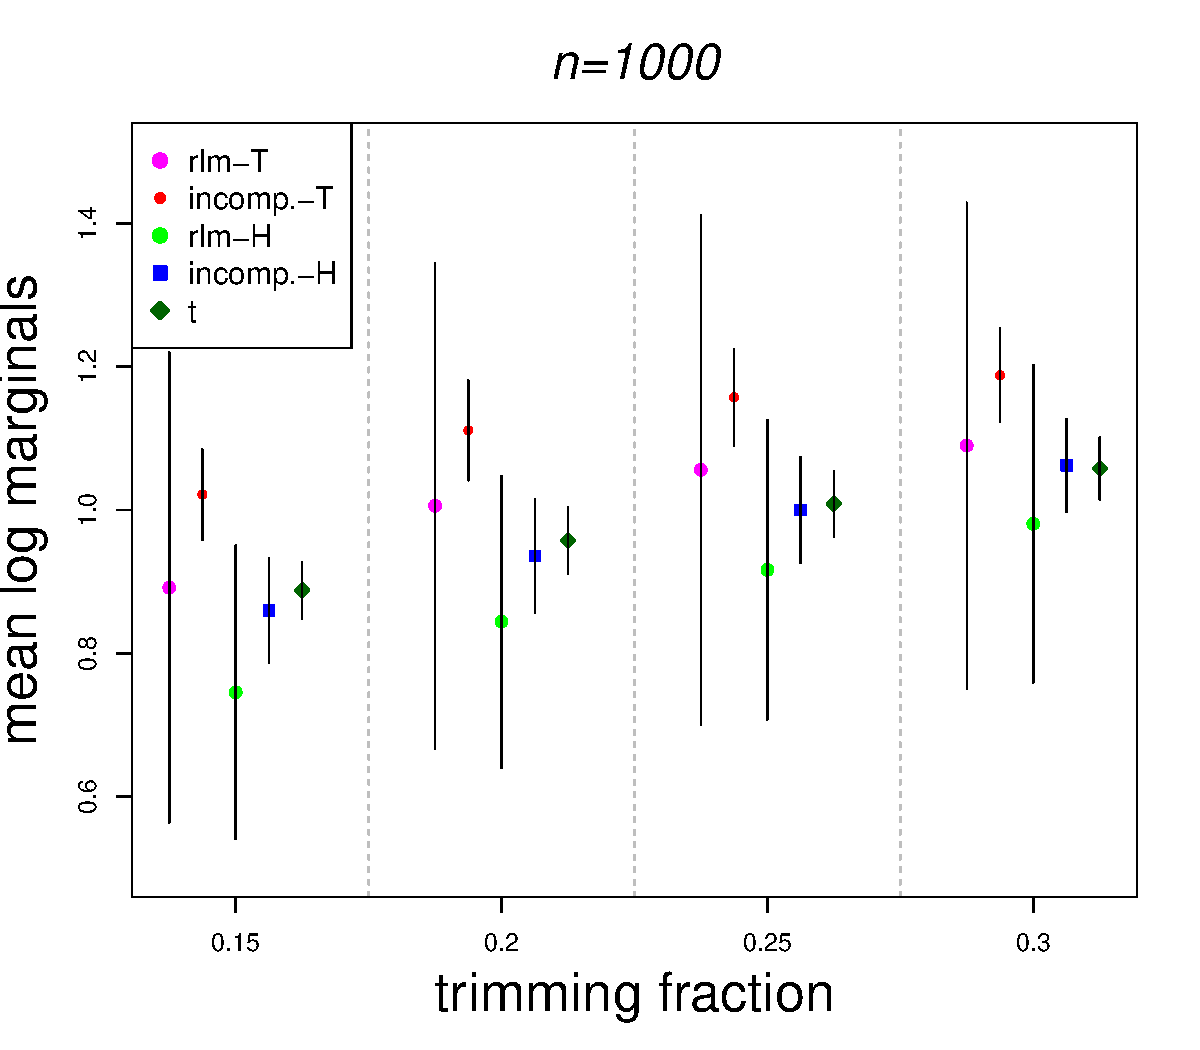
\includegraphics[width=2.75in,page=1]{hierlogMargType1AgenciesBaseModelt}}\quad
%%\subcaptionbox{}{\includegraphics[width=2.75in,page=2]{hierlogMargType1AgenciesBaseModelt}}
%\subcaptionbox{}{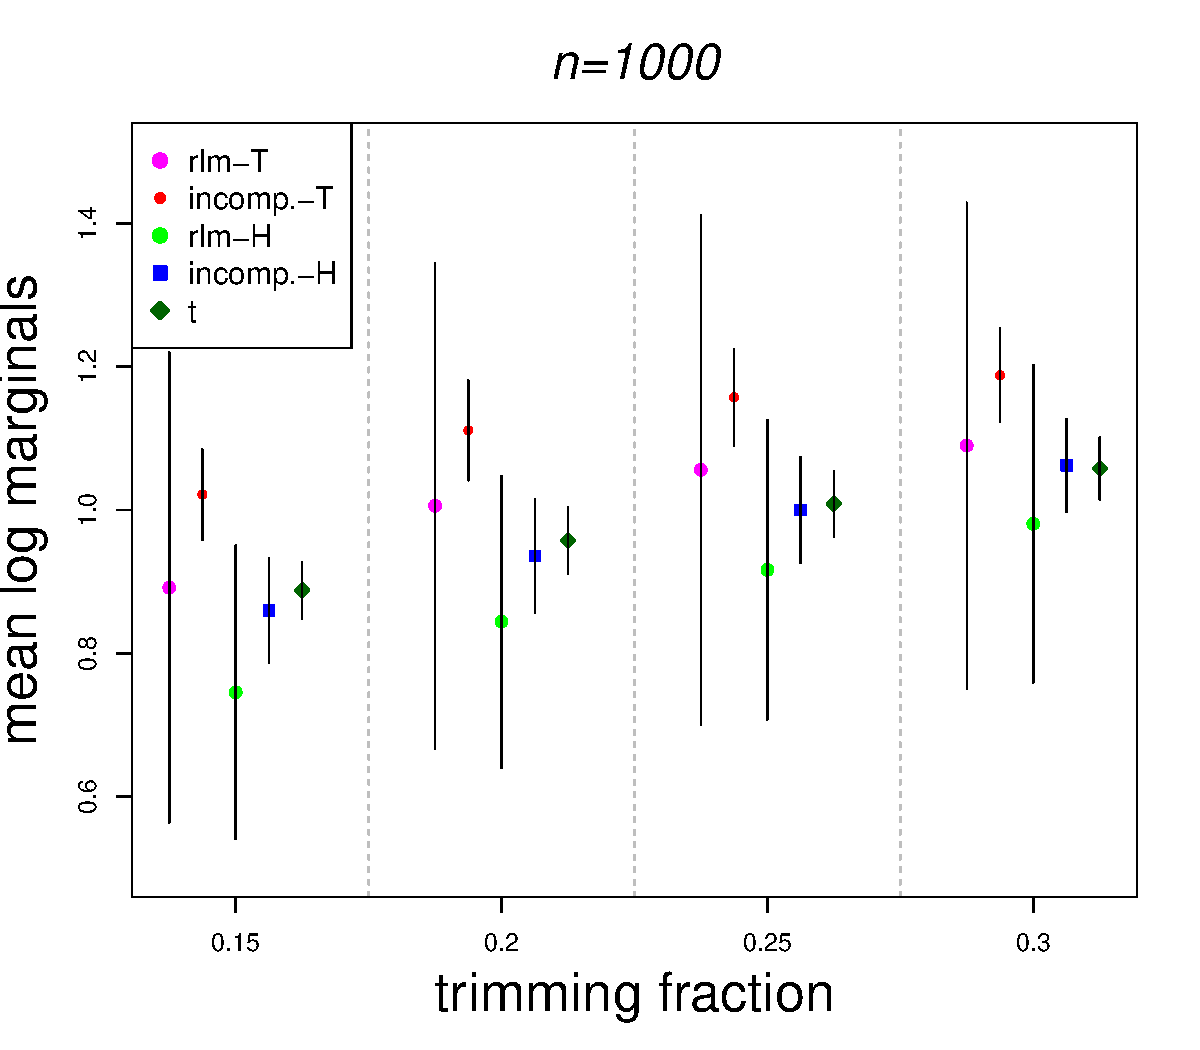
\includegraphics[width=4in,page=1]{hierlogMargType1AgenciesBaseModelt}}\quad
%\subcaptionbox{}{\includegraphics[width=4in,page=2]{hierlogMargType1AgenciesBaseModelt}}
%\caption{Model evaluation for `Type 1' agencies under the hierarchical model for $n=1000$ and $2000$. The $t$-model is used as the base method to compute TLM. Plotted are the mean TLM for each model against the trimming fraction across the $100$ cross-validation samples. Error bars correspond to one standard deviation of TLM above and below the mean. Models are labeled using the same notation as the previous figure. Only the relevant trimming fractions ($\alpha\geq .15$) are pictured.  
%}
%\label{fig:hierType1Marg}
%\end{sidewaysfigure}



\subsection{Comparison of hierarchical and non-hierarchical fits}

The performance of the methods for the hierarchical and non-hierarchical models can be contrasted through our cross validations studies.  We focus on Tukey's and Huber's conditioning statistic and concentrate our evaluation on the `Type 1' agencies. Table~\ref{tab:tlmTable} displays the mean TLM for each model and range of trimming fractions.  Our summary below focuses exclusively on realistic trimming fractions, $\alpha \geq 0.15$, and Tukey's conditioning statistic.  

We first note that for the non-hierarchical model, there is little difference between mean TLM for $n=1000$ and $n=2000$, with 
the numbers differing only in the third decimal place (see rows 1 and 3 of the table).  This is due to the posterior predictive distributions having stabilized.  The
mean TLMs for the hierarchical model show a greater change with increases of about $0.05$ to $0.08$ as the training sample size changes
from $1000$ to $2000$ (see rows 2 and 4 of the table).  For calibration, the mean TLM for a normal with mean $0.5$ and variance $1$ is approximately this size
when trimming is done under a standard normal base model.  Thus, the increase in mean TLM is substantial.  
We attribute the change for the hierarchical model to the 
improvement in fits, particularly for states with fewer agencies.  

Direct comparison of the hierarchical and non-hierarchical models shows that, for $n=1000$, the non-hierarchical model has uniformly 
(for $\alpha$ of interest) better mean TLM (rows 1 and 2).  The differences are substantial, and the summaries primarily reflect greater stability of fits on a state-by-state basis under the non-hierarchical model.  To a lesser extent, they reflect variation in the evaluation criterion which stems from modest validation sample size, particularly with larger trimming fractions.  The trimmed cases are not proportionally distributed across states.  The pattern changes for $n=2000$ (rows 3 and 4), with the hierarchical model showing larger mean TLMs for trimming fractions $0.15$ and $0.20$.  The improvement reflects the ability of the hierarchical model to capture differences in regressions across the states which is realized when the training sample size is large enough.  We attribute the better performance of the non-hierarchical model for the largest trimming fractions to variation in the evaluation.  

\begin{table}[!tbp]
{\small
\begin{center}
\begin{tabular}{lllll}
\hline\hline
& \multicolumn{4}{c}{Trimming fraction ($\alpha$)}\\
\multicolumn{1}{l}{}&\multicolumn{1}{c}{$0.15$}&\multicolumn{1}{c}{$0.2$}&\multicolumn{1}{c}{$0.25$}&\multicolumn{1}{c}{$0.3$}\tabularnewline
\hline
{\mdseries Tukey ($n=1000$)}&&&&\tabularnewline
~~Non-Hier.&1.072 (0.014)&1.179 (0.022)&1.226 (0.029)&1.255 (0.033)\tabularnewline
~~Hier.&1.021 (0.063)&1.110 (0.070)&1.157 (0.067)&1.187 (0.065)\tabularnewline
\hline
{\mdseries Tukey ($n=2000$) }&&&&\tabularnewline
~~Non-Hier.&1.068 (0.029)&1.178 (0.007)&1.225 (0.011)&1.254 (0.014)\tabularnewline
~~Hier.&1.094 (0.041)&1.189 (0.036)&1.221 (0.033)&1.242 (0.028)\tabularnewline
\hline
{\mdseries Huber  ($n=1000$)}&&&&\tabularnewline
~~Non-Hier.&1.020 (0.020)&1.114 (0.035)&1.157 (0.041)&1.184 (0.045)\tabularnewline
~~Hier.&0.861 (0.073)&0.937 (0.079)&1.001 (0.074)&1.063 (0.064)\tabularnewline
\hline
{\mdseries Huber ($n=2000$)}&&&&\tabularnewline
~~Non-Hier.&1.015 (0.021)&1.112 (0.014)&1.154 (0.019)&1.181 (0.023)\tabularnewline
~~Hier.&0.930 (0.041)&1.014 (0.043)&1.080 (0.035)&1.148 (0.027)\tabularnewline
\hline
\end{tabular}
\end{center}
\caption{Mean (standard deviation) of TLM for `Type 1' agencies for the Bayesian restricted likelihood non-hierarchical and hierarchical models for $n=1000$ and $2000$.} \label{tab:tlmTable}
}
\end{table}


\section{Discussion}
\label{Conclusions}

%In this work, we have presented an approach which begins to reconcile Bayesian methods with the practice of data analysis.
Many routine choices in an analysis react to the gap between reality and the
statistical model, where a bit of set-up work improves inferential
performance.  Often, these choices can be recast in the framework of
restricted likelihood presented here, lending them more formality and facilitating
development of theoretical results.  But a much greater benefit of our
framework is that it leads us to blend classical estimation with
Bayesian methods.  Here, we use the likelihood from robust regression
estimators to move from prior distribution to posterior distribution.
Conditioning on the estimator, the update follows Bayes' Theorem
exactly.   Computation is driven by MCMC methods, requiring only a modest supplement to existing algorithms.  In another context, we might condition on the results of a set of estimating equations, designed to enforce lexical preferences for those features of the analysis considered most important, yet still producing inferences for secondary aspects of the problem. For example, the computational strategies we devised here allow us to apply the method to inference on quantiles of a regression model. In other settings, we envision conditioning on a mix of estimators and some of the observed data.  

The framework we propose allows us to retain many benefits of Bayesian methods:  it requires a full and complete model for the data; it lets us combine various sources of information both through the use of a prior distribution and through creation of a hierarchical model; it guarantees admissibility of our decision rules among the class based on the summary statistic $T(\by)$; and it naturally leads us to focus on predictive inference.   

This same framework retains many of the benefits of classical estimation.  Great ingenuity has been used to create a wide variety of estimators in this tradition, many of which are designed to handle specific flaws in the model.  The estimators are typically accompanied by asymptotic results on consistency and distribution.  Many of these results carry over to our blend of classical and Bayesian methods, although regularity conditions differ.  We expect our procedures to have strong large sample performance, especially in settings where
pooling of information is of value.  

This framework opens a number of questions, including a need to revisit such issues as model selection, model averaging for predictive performance, and the role of diagnostics.  Perhaps the biggest question is which summary statistic to choose.  For this, we recommend a choice based on the analyst's understanding of the problem, model, reality, deficiencies in the model,  inferences to be made, and the relative importance of various inferences.  \green{In our words, to provide desireable inference, we recommend use of robust and relevant summary statistics in conjunction with Bayesian models.}  


\section{Appendix}
\label{sec:appendix}

\subsection{Details of Examples in Section \ref{examples}}
\subsubsection{Speed of Light}
With parameters $\beta$ and $\sigma$, the full model is $\beta\sim N(23.6, 2.04^{2})$, $\sigma^{2}\sim IG(5, 10)$, $y_{i}\iid N (\beta, \sigma^{2})$ for $i=1,2,\dots, n=66$ where $y_{i}$ denotes the $i^{th}$ measurement of the passage time of light. $\beta$ is interpreted as the passage time of light with
$\sigma^{2}$ representing measurement error. Tuning parameters for the M-estimators are chosen to achieve $95\%$ efficiency under normality and for comparability, roughly $5\%$ of the residuals are trimmed for LTS.  The t-model assumes $y_{i}\iid t_{\nu} (\beta, \sigma^{2})$ with $\nu=5$. The prior on $\sigma^{2}$ is $IG(5, \frac{\nu-2}{\nu}10)$ so the prior on the variance is the same as the other models. %We note that the variance of the data under this model is $\frac{\nu}{\nu-2}\sigma^{2}$.  For comparability, it is this quantity that has the prior distribution $IG(a,b)$ given above.   \citep[for details see][]{huber2009}

\subsubsection{Belgium Calls}
With $\bbeta = (\beta_{0}, \beta_{1})^{\top}$ and $\sigma$ the full model is $\bbeta\sim N(\boldmath{\mu}_{0}, \boldmath{\Sigma}_{0})$, $\sigma^{2} \sim IG(a, b)$, $\by \sim N(X\bbeta, \sigma^{2} I)$. Where $\mb y$ is the vector of the logarithm of the number of calls. Maximum likelihood estimators fit to the first three data points is used to set the prior parameters. In particular, $\Sigma_{0} = g\sigma_{0}^2 (X^{\top}X)^{-1}$ and $\mu_{0} = (1.87,  0.03)^{\top}$, $\sigma_{0} = 0.03$ the MLEs fit to the first three data points. The models are fit to the remaining 21 data points and the parameter $g$ is set to $21$ reflecting a unit information prior \cite{}. Finally $a = 2$ and $b =1$ for the normal theory and restricted likelihood models. For the t-model,  $\by \sim t_{\nu}(X\bbeta, \sigma^{2} I)$ with degrees of freedom set to $\nu = 5$ and the scale of the inverse gamma prior on the $\sigma^{2}$ adjusted to $\frac{\nu-2}{\nu}$ so the prior on the variance is the same as the other models.

\subsection{Proofs}
\noindent

Proof of Theorem~\ref{Transformation}.  
\begin{proof} 
\begin{eqnarray}
 s(X,\by) & = & s\left(X,\frac{s(X,\by_{obs})}{s(X,\bz^*)}\bz^* + X\left(\bb(X,\by_{obs}) - \bb(X,\frac{s(X,\by_{obs})}{s(X,\bz^*)}\bz^*)\right)\right) \\
& = & \frac{s(X,\by_{obs})}{s(X,\bz^*)} s(X, \bz^*)= s(X,\by_{obs}) , \qquad \mbox{and} \\
 \bb(X,\by) & = & \bb\left(X,\frac{s(X,\by_{obs})}{s(X,\bz^*)}\bz^* + X\left(\bb(X,\by_{obs}) - \bb(X,\frac{s(X,\by_{obs})}{s(X,\bz^*)}\bz^*)\right)\right) \\
 & = & \bb(X,\frac{s(X,\by_{obs})}{s(X,\bz^*)}\bz^*) + \bb(X,\by_{obs}) - \bb(X,\frac{s(X,\by_{obs})}{s(X,\bz^*)}\bz^*) \\ &=& \bb(X,\by_{obs})
\end{eqnarray}
\end{proof}

\noindent
Proof of Lemma~\ref{gradSTheoremReg}.
\begin{proof}
We first show that $\nabla s(X,\by)\in \mc{C}^\perp(X)$. Recall that
$H=I-Q$. By the regression invariance property \ref{regIn} of $s$, we have
\label{perpGradReg}
\begin{equation}
\label{eq:lem3.2}
\begin{aligned}
s(X,\by)=s(X, Q\by+H\by)=s(X, Q\by).
\end{aligned}
\end{equation}
Thus, by the chain rule $\nabla s(X,\by)=Q\nabla s(X,Q\by)=Q\nabla s(X, \bz)$. Hence $X^\top \nabla s(X,\by)=0$ as desired.
From equation~\eqref{eq:lem3.2}, all vectors $\bz'\in \Pi(\mathcal{A})$ satisfy $s(X,\bz')=
s(X,\by)=s(X,\by_{obs})$, and so all directional derivatives of $s$ along each tangent $\bv$ to
  $\Pi(\mathcal{A})$ in $\mc C^\perp(X)$ at $\bz$ are equal to 0 (i.e., $\nabla s(X,\bz) \cdot \bv=0$).  Thus $\nabla s(X,\bz)$ is orthogonal to  $\Pi(\mathcal{A})$ at $\bz$.  
Since $\Pi(\mathcal{A})$ has dimension $n-p-1$, $\nabla s(X,\bz)$ gives the unique (up to scaling and reversing direction) normal in the $n-p$ dimensional $\mc C^\perp(X)$.  
\end{proof}

\noindent
Proof of Lemma~\ref{lem:basis}

\begin{proof}
Without loss of generality, assume the columns of $X$ form an
orthonormal basis for $\mc C (X)$ and likewise the columns of $W$ form
and orthonormal basis for $\mc C^\perp(X)$. With earlier notation,
$H=XX^{\top}$ and $Q=WW^{\top}$. The set $\mc A$ is defined by the
$p+1$ equations  $s(X,\by)=s(X,\by_{obs})$, 
$b_1(X,\by)=b_1(X,\by_{obs}),\dots,  b_p(X,\by)=b_p(X,\by_{obs})$. Consequently, the gradients are orthogonal to $\mc A$. Let  $\nabla\bb(X,\by)$ denote the $n\times p$ matrix with columns $\nabla b_1(X,\by),\dots, \nabla b_p(X,\by)$. We seek to show the $n \times (p+1)$ matrix $[\nabla\boldsymbol\bb(X,\by),\nabla s(X,\by)]$ has rank $p+1$. Using property \ref{regEq}, we have that 
\[
\bb(X, \by)=\bb(X,Q\by+H\by)=\bb(X, Q\by)+X^\top \by
\] 
Then $\nabla \bb(X,\by)=Q\nabla\boldsymbol\bb(X, Q\by)+ X$ and 
\begin{eqnarray}
\label{BigMatrix}
[XX^\top, WW^\top]^\top[\nabla\boldsymbol\bb(X,\by),\nabla s(X,\by)]=
 \left( \begin{array}{cc}
X & \mathbf{0} \\
WW^\top\nabla b(X,\by)  &\nabla s(X,\by)  \\ \end{array} \right)
\end{eqnarray}
The last column comes from Lemma \ref{gradSTheoremReg}. The matrix $[XX^\top, WW^\top]^\top$ is of full
column rank (rank $n$), and so the rank of $[\nabla\boldsymbol\bb(X,\by),\nabla s(X,\by)]$ is the same as the rank
of the matrix on the right hand side of (\ref{BigMatrix}).  This last
matrix has rank $p+1$ since $\nabla s(X,\by) \ne \bzero$ by \ref{scaleEq2Reg}, and so does 
$[\nabla b(X,\by),\nabla s(X,\by)]$.
\end{proof}

\noindent
Proof of Lemma~\ref{lem:fullrank}

\begin{proof}
$P$ is the projection of the columns of $A$ onto $\mc
C^{\perp}(X)$. For this to result in a loss of rank, a subspace of
$\mc T_{y}(\mc A)$ must belong to $\mc C(X)$.  Following property
\ref{regEq}, for an arbitrary vector $X \bv \in \mc C(X)$, $\bb(X,\by
+ X \bv) = \bb(X,\by) + \bv$.  From the property, we can show that the directional derivative
  of $\bb$ along $X \bv$ with $\bv \ne \bzero$ is $\bv$, which is a
  nonzero vector. Hence $X\bv \notin \mc T_{y}(\mc A)$.  
\end{proof}

\noindent
Proof of Corollary~\ref{theorem:sings}

\begin{proof}
The corollary relies on a lemma and theorem from \cite{miao1992} which we restate 
slightly for brevity of presentation.  The principal angles between subspaces pluck off a
set of angles between subspaces, from smallest to largest.  The number of such angles 
is the minimum of the dimensions of the two subspaces.  Miao and Ben-Israel's first result
(their Lemma 1) connects these principal angles to a set of singular values, and hence to 
volumes.   
\begin{lemma}{(Miao, Ben-Israel)}
\label{MBI:lemma}
Let the columns of $Q_L\in \mathbb{R}^{n\times l}$ and $Q_M\in
\mathbb{R}^{n\times m}$ form orthonormal bases for linear subspaces
$L$ and $M$ respectively, with $l \leq m$. Let $\sigma_1\geq\cdots\geq
\sigma_l\geq0$ be the singular values of $Q_M^\top Q_L$. Then $\cos
\theta_i=\sigma_i, i=1,\dots,l$ where $0\leq\theta_1\leq\theta_2\leq
\cdots \leq\theta_l\leq\frac{\pi}{2}$ are the principal angles between $L$ and $M$.  
\end{lemma}

Miao and Ben-Israel's second result (their Theorem 3) makes a match between the principal
angles between a pair of subspaces and the principal angles between their orthogonal complements.  
\begin{theorem}{(Miao, Ben-Israel)}
\label{MBI:thm}
The nonzero principal angles between subspace $L$ and $M$ are equal to the 
nonzero principal angles between $L^\perp$ and $M^\perp$.
\end{theorem}

To establish the corollary, we appeal to Lemma~\ref{MBI:lemma} and Theorem~\ref{MBI:thm}.  Translating Miao and Ben Israel's
notation, we have $M=\mc C^\perp (X)$, $Q_M=W$, $L=\mc
T_{\boldsymbol{y}}(\mc{A})$, and $Q_L= A$. By Theorem~\ref{MBI:thm}, the
nonzero principal angles between $\mc{T}_{\boldsymbol{y}}(\mc{A})$ and
$\mc C^\perp(X)$ are the same as the nonzero principal angles between
$\mathcal{T}_{\boldsymbol{y}}^\perp(\mathcal{A})$ and $\mc C(X)$. By
\ref{MBI:lemma}, the non-unit singular values of $W^\top A$ are the
same as the non-unit singular values of $U^\top B$.  
\end{proof}

\subsection{Setting the hierarchical prior values}
In setting the priors we use the same previous data set used to set the priors for the non-hierarchical model (Section \ref{regModelNW}) and several heuristic arguments. While the analyses in Section \ref{hierRegNW} set the hyper-parameters using what is described here, the results were not sensitive to these choices.  This section describes the heuristics used in setting these prior parameters and is given for completeness. Using the previous data set we fit separate (robust) regressions to each state and a  regression to the \green{\sout{entire} entirety of the} data at once. Let the estimates for the fits to each state be $\hat{\beta_{1}}, \dots, \hat \beta_{J}, \hat \sigma_{1}, \dots, \hat \sigma_{J}$ and the estimates from the single regression be $\hat \beta$ and $\hat \sigma$. These are classical robust estimates using Tukey's regression and Huber's scale. Let $n_{j}$ denote the number of observations in the $j^{th}$ state and set $n=\sum n_{j}$. 

First, consider $v_{1}$ and $v_{2}$ in the prior $b\sim\text{beta}(v_{1},v_{2})$.  In the hierarchical model \eqref{eq:hierModel}, $b=0$ implies all the $\bbeta_{j}'s$ are equal (no variation between states) and $b=1$ implies the $\bbeta_{j}'s$ vary about $\mu_{0}$ according to $\Sigma_{0}=n\cdot \mbox{var}(\hat\beta)$ (see Section \ref{regModelNW}). We seek a prior measure for what we think $b$ should be. In other words, how much prior uncertainty should we allow in $\bbeta$ as opposed to the uncertainty amongst the $\bbeta_{j}'s$? Using the prior fit, a measure for  uncertainty for $\bbeta$ is $\Sigma_{\hat\beta}=\mbox{var}(\hat\beta)$, the estimate of the covariance from the single regression. For the $\bbeta_{j}'s$, take $\delta_{j}=\hat\beta_{j}-\hat\beta$ and set the prior uncertainty to $\Sigma_{\delta}=n^{-1}\sum n_{j}\delta_{j}\delta_{j}^{\top}$. Consider the value $g= \left(|\Sigma_{\delta}|/|\Sigma_{\hat\beta}|\right)^{1/p}$. Heuristically, $g$ is measure of the amount of uncertainty between the $\bbeta_{j}'s$ to the amount of uncertainty in $\bbeta$. Now in the prior, we heuristically set the uncertainty in the $\bbeta_{j}'s$ ($b\Sigma_{0}$) to be approximately equal to $g\cdot\mbox{var}(\hat\beta)$. That is, $b\Sigma_{0}\approx g\cdot\mbox{var}(\hat\beta)= \frac{g}{n} \Sigma_{0}$, suggesting $b\approx  \frac{g}{n}$.  Hence we set $E[b]=\frac{g}{n}$. The precision, $v_{1}+v_{2}$, is set to be relatively high at $20$, completing the specification for the prior on $b$. 

In setting the parameters for the beta prior on $\mu_{\rho}$ and gamma prior on  $\psi_\rho$ we first take $\hat z_{j}= \Phi^{-1} (H(\hat\sigma_{j}^{2}))$. As in the prior we assume $(\hat z_1,\dots,\hat z_J)\sim N_J(\mathbf{0}, \Sigma_\rho)$ with
$\Sigma_\rho=(1-\rho)I+\rho \mb{1}\mb{1}^{\top}$ and find the MLE, $\hat\rho_{mle}$, and observed inverse Fisher information, $I^{-1}(\rho_{mle})$. The mean of the beta prior on $\mu_{\rho}$ is set to $\hat\rho_{mle}$. Its variance is inflated somewhat and set to $2I^{-1}(\hat\rho_{mle})$. Since $\text{var}(\rho|\mu_{\rho}, \psi_{\rho})=\mu_{\rho} (1-\mu_{p})/(\psi_{\rho}+1)$ we replace $\mu_{\rho}$ with $\hat\rho_{mle}$, $\text{var}(\rho|\mu_{\rho}, \psi_{\rho})$ with $2I^{-1}(\hat\rho_{mle})$, and set the mean of the gamma prior on $\psi_{\rho}$ equal to $\hat\rho_{mle} (1-\hat\rho_{mle})/(2I^{-1}(\hat\rho_{mle}))-1$. Finally, we arbitrarily set the variance of the gamma prior to be approximately the same as the mean.
%The variance was set to twice the inverse Fisher information evaluated at $\hat\rho_{mle}$

%
%Plugging the estimates of $z_j$ into the multivariate normal, the mean of $\mu_\rho$ is set to the MLE of $\rho$ and the variance is set to the observed inverse Fisher information matrix, inflated by a factor of $2$ to weaken the prior for this parameter.  We use the same MLE and inflated information matrix to set the mean for $\psi_{\rho}$. Its variance is chosen to cover a range of plausible values. A range of other values for the fixed hyper-parameters was also studied.  The differences in results were negligible. 


\bibliographystyle{apalike}
\bibliography{refs}

\end{document}



